\documentclass[11pt,a4paper]{article}
\usepackage[margin=1.9cm, top=2.1cm, bottom=2.0cm]{geometry}
\usepackage[T1]{fontenc}
\usepackage{lmodern}
\usepackage{amsmath,amssymb}
\usepackage{enumitem,booktabs,array,tabularx,multirow}
\usepackage[normalem]{ulem}
\usepackage{adjustbox}
\usepackage{xcolor}
\usepackage{fancyhdr,lastpage}
\usepackage[most]{tcolorbox}
\usepackage{tikz}
\usetikzlibrary{shapes.geometric,arrows.meta,positioning,calc}
\usepackage[hidelinks]{hyperref}
\setlength{\parindent}{0pt}
\setlength{\parskip}{4pt}
\renewcommand{\arraystretch}{1.25}
\emergencystretch=2em
\pagestyle{fancy}\fancyhf{}
\lhead{\small\textit{Course: CS420 -- Artificial Intelligence}}
\rhead{\small Practice Test 3 -- Solution}
\cfoot{\small Page \thepage\ of \pageref{LastPage}}
\renewcommand{\headrulewidth}{0.4pt}
% empty answer box (exam) / filled box (solution)
\newtcolorbox{ansbox}[1][]{enhanced, breakable, colback=white, colframe=black!55, boxrule=0.5pt, arc=0pt,
  left=5pt, right=5pt, top=3pt, bottom=3pt, before skip=3pt, after skip=6pt, #1}
\newtcolorbox{solbox}{enhanced, breakable, colback=blue!2!white, colframe=blue!50!black, boxrule=0.6pt, arc=0pt,
  left=6pt, right=6pt, top=4pt, bottom=4pt, before skip=3pt, after skip=8pt,
  fontupper=\color{black}}
\newcommand{\question}[1]{\par\medskip\noindent\textbf{Question #1.}\ }
\newcommand{\subq}[1]{\par\smallskip\noindent\textbf{#1}\ }
\newcommand{\T}{\textbf{\textcolor{green!45!black}{TRUE}}}
\newcommand{\F}{\textbf{\textcolor{red!70!black}{FALSE}}}

\tikzset{
  maxn/.style={draw, thick, regular polygon, regular polygon sides=3, minimum size=10.5mm, inner sep=0pt, font=\small},
  minn/.style={maxn, shape border rotate=180},
  chn/.style={draw, thick, circle, minimum size=9.5mm, inner sep=0pt, font=\small},
  leafn/.style={draw, rectangle, minimum width=5.5mm, minimum height=5.5mm, inner sep=1pt, font=\small},
  gone/.style={draw=black!25, text=black!35},
  cut/.style={red!80!black, very thick, dashed},
  sol/.style={text=blue!70!black, font=\small\bfseries},
}

\begin{document}


{\large\textbf{\textit{Course: CS420 -- Artificial Intelligence}}}\par
{\textbf{\textit{Midterm examination review -- Lectures 0 to 3}}}\par
\begin{center}{\Large\bfseries PRACTICE MIDTERM EXAMINATION -- TEST 3\\[2pt]\textcolor{blue!55!black}{SOLUTION}}\\[3pt]
{\small Duration: 120 minutes \quad$\cdot$\quad Closed book \quad$\cdot$\quad Calculator allowed}\end{center}
\noindent\rule{\linewidth}{0.6pt}

{\small\textit{Unless a question says otherwise, ties are broken in alphabetical order (left-to-right in trees), and successors are generated in alphabetical order.}}\par
\question{1}\textit{Tower of Hanoi with 3 pegs and 3 disks.} Three disks of different sizes are stacked on peg 1 (largest at the bottom). The goal is to move the stack to peg 3, moving one disk at a time and never placing a larger disk on a smaller one.
\subq{(a)}Consider a state as a tuple of values. Which values should be included in the tuple?
\begin{solbox}
$(p_1,p_2,p_3)$ = the peg of the small, medium and large disk. On a peg the order of the disks is forced by their sizes, so it does not need to be stored.
\end{solbox}
\subq{(b)}Define the initial state and the goal state.
\begin{solbox}
Initial $(1,1,1)$; goal $(3,3,3)$.
\end{solbox}
\subq{(c)}Define the action function.
\begin{solbox}
Move the top disk of peg $a$ (the smallest $i$ with $p_i=a$) to peg $b\neq a$, provided peg $b$ is empty or its top disk is larger; the result sets $p_i=b$.
\end{solbox}
\subq{(d)}What is the action cost?
\begin{solbox}
1 per move.
\end{solbox}
\subq{(e)}What is the maximum number of states? How many are reachable? What is the length of an optimal solution?
\begin{solbox}
$3^3=\mathbf{27}$ tuples; every tuple is legal and all \textbf{27} are reachable. Optimal solution: $2^3-1=\mathbf{7}$ moves.
\end{solbox}
\question{2}Consider the undirected graph below; $S$ is the initial state and $G$ the goal state. \begin{center}
\begin{adjustbox}{max width=\linewidth}
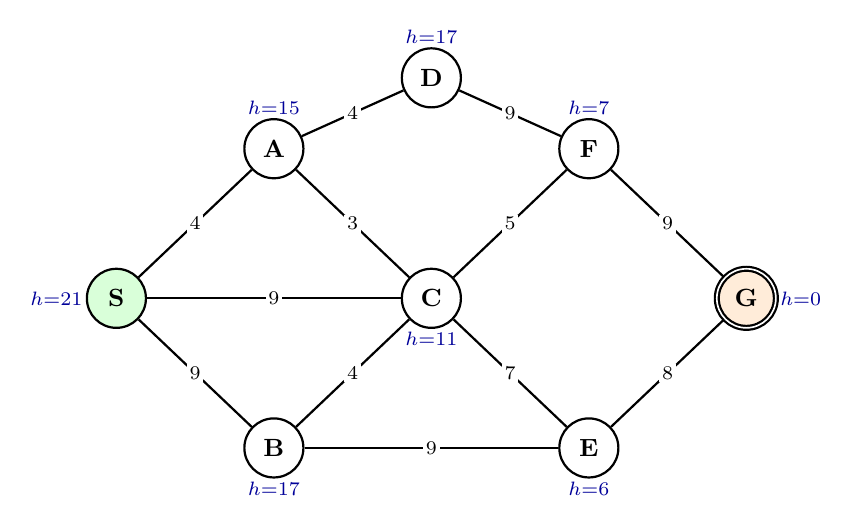
\begin{tikzpicture}[scale=1.0, every node/.style={transform shape}, gn/.style={draw, thick, circle, minimum size=7.5mm, inner sep=0pt, font=\small\bfseries}, ec/.style={font=\scriptsize, fill=white, inner sep=1pt}]
\node[gn, fill=green!15, label={[font=\scriptsize, text=blue!60!black, inner sep=1pt]left:$h{=}21$}] (S) at (0.00,0.00) {S};
\node[gn, label={[font=\scriptsize, text=blue!60!black, inner sep=1pt]above:$h{=}15$}] (A) at (2.00,1.90) {A};
\node[gn, label={[font=\scriptsize, text=blue!60!black, inner sep=1pt]below:$h{=}17$}] (B) at (2.00,-1.90) {B};
\node[gn, label={[font=\scriptsize, text=blue!60!black, inner sep=1pt]below:$h{=}11$}] (C) at (4.00,0.00) {C};
\node[gn, label={[font=\scriptsize, text=blue!60!black, inner sep=1pt]above:$h{=}17$}] (D) at (4.00,2.80) {D};
\node[gn, label={[font=\scriptsize, text=blue!60!black, inner sep=1pt]below:$h{=}6$}] (E) at (6.00,-1.90) {E};
\node[gn, label={[font=\scriptsize, text=blue!60!black, inner sep=1pt]above:$h{=}7$}] (F) at (6.00,1.90) {F};
\node[gn, double, fill=orange!15, label={[font=\scriptsize, text=blue!60!black, inner sep=1pt]right:$h{=}0$}] (G) at (8.00,0.00) {G};
\draw[thick] (S) to[] node[ec, midway]{4} (A);
\draw[thick] (S) to[] node[ec, midway]{9} (B);
\draw[thick] (S) to[] node[ec, midway]{9} (C);
\draw[thick] (A) to[] node[ec, midway]{3} (C);
\draw[thick] (A) to[] node[ec, midway]{4} (D);
\draw[thick] (B) to[] node[ec, midway]{4} (C);
\draw[thick] (B) to[] node[ec, midway]{9} (E);
\draw[thick] (C) to[] node[ec, midway]{5} (F);
\draw[thick] (C) to[] node[ec, midway]{7} (E);
\draw[thick] (D) to[] node[ec, midway]{9} (F);
\draw[thick] (E) to[] node[ec, midway]{8} (G);
\draw[thick] (F) to[] node[ec, midway]{9} (G);
\end{tikzpicture}
\end{adjustbox}
\end{center}For each search strategy, (a) list, in order, the states \textbf{expanded}, (b) give the path found and (c) give the final content of the frontier (a state is expanded when it is removed from the frontier). Conventions: BFS, DFS and greedy best-first search test a state for the goal when it is \emph{generated} (so the goal is not expanded); UCS and A* test it when it is \emph{removed} from the frontier (graph search; a cheaper path to a frontier state replaces its entry). DFS avoids loops by remembering the states on the current path only. The path returned will not be accepted if the list of expanded states is wrong.

\begin{solbox}
\begin{center}\small\begin{tabularx}{\linewidth}{|>{\raggedright}p{2.6cm}|>{\raggedright}X|>{\raggedright}p{3.6cm}|>{\raggedright\arraybackslash}p{2.6cm}|}\hline
\textbf{Algorithm} & \textbf{List of expanded states} & \textbf{Path returned} & \textbf{Final frontier}\\ \hline
Breadth-first search & \textcolor{blue!60!black}{S A B C D E} & \textcolor{blue!60!black}{S B E G} (cost 26) & \textcolor{blue!60!black}{$\{$ F $\}$}\\ \hline
Uniform-cost search & \textcolor{blue!60!black}{S A C D B F E G} & \textcolor{blue!60!black}{S A C F G} (cost 21) & \textcolor{blue!60!black}{$\{\ \}$}\\ \hline
Depth-first search & \textcolor{blue!60!black}{S A C B E} & \textcolor{blue!60!black}{S A C B E G} (cost 28) & \textcolor{blue!60!black}{(not asked)}\\ \hline
Greedy best-first search & \textcolor{blue!60!black}{S C E} & \textcolor{blue!60!black}{S C E G} (cost 24) & \textcolor{blue!60!black}{$\{$ F, A, B $\}$}\\ \hline
Graph-search A* & \textcolor{blue!60!black}{S A C F E G} & \textcolor{blue!60!black}{S A C F G} (cost 21) & \textcolor{blue!60!black}{$\{$ D, B $\}$}\\ \hline
\end{tabularx}\end{center}\textbf{BFS} (queue after each expansion):\begin{center}\small\begin{tabularx}{\linewidth}{c c >{\raggedright\arraybackslash}X}\toprule
Step & Expanded & Queue (front $\rightarrow$ back) after the expansion \\ \midrule
1 & S & A, B, C \\
2 & A & B, C, D \\
3 & B & C, D, E \\
4 & C & D, E, F \\
5 & D & E, F \\
6 & E & generates goal \textbf{G} $\Rightarrow$ stop; frontier: F \\
\bottomrule\end{tabularx}\end{center}\textbf{DFS} (stack after each expansion):\begin{center}\small\begin{tabularx}{\linewidth}{c c >{\raggedright\arraybackslash}X}\toprule
Step & Expanded & Stack (top $\rightarrow$ bottom) after the expansion \\ \midrule
1 & S & A, B, C \\
2 & A & C, D, B, C \\
3 & C & B, E, F, D, B, C \\
4 & B & E, E, F, D, B, C \\
5 & E & generates goal \textbf{G} $\Rightarrow$ stop; frontier: E, F, D, B, C \\
\bottomrule\end{tabularx}\end{center}\textbf{UCS:}\begin{center}\small\begin{tabularx}{\linewidth}{c l >{\raggedright\arraybackslash}X}\toprule
Step & Expanded & Frontier after the expansion, in priority order (subscript $=g(n)$) \\ \midrule
1 & S$_{0}$ & A$_{4}$, B$_{9}$, C$_{9}$ \\
2 & A$_{4}$ & C$_{7}$, D$_{8}$, B$_{9}$ \\
3 & C$_{7}$ & D$_{8}$, B$_{9}$, F$_{12}$, E$_{14}$ \\
4 & D$_{8}$ & B$_{9}$, F$_{12}$, E$_{14}$ \\
5 & B$_{9}$ & F$_{12}$, E$_{14}$ \\
6 & F$_{12}$ & E$_{14}$, G$_{21}$ \\
7 & E$_{14}$ & G$_{21}$ \\
8 & G$_{21}$ & \textit{goal removed from the frontier -- stop} \\
\bottomrule\end{tabularx}\end{center}\textbf{Greedy best-first:}\begin{center}\small\begin{tabularx}{\linewidth}{c l >{\raggedright\arraybackslash}X}\toprule
Step & Expanded & Frontier after the expansion, in priority order (subscript $=h(n)$) \\ \midrule
1 & S$_{21}$ & C$_{11}$, A$_{15}$, B$_{17}$ \\
2 & C$_{11}$ & E$_{6}$, F$_{7}$, A$_{15}$, B$_{17}$ \\
3 & E$_{6}$ & generates goal \textbf{G} $\Rightarrow$ stop; frontier: F$_{7}$, A$_{15}$, B$_{17}$ \\
\bottomrule\end{tabularx}\end{center}\textbf{A*:}\begin{center}\small\begin{tabularx}{\linewidth}{c l >{\raggedright\arraybackslash}X}\toprule
Step & Expanded & Frontier after the expansion, in priority order (subscript $=g+h=f$) \\ \midrule
1 & S$_{0+21=21}$ & A$_{4+15=19}$, C$_{9+11=20}$, B$_{9+17=26}$ \\
2 & A$_{4+15=19}$ & C$_{7+11=18}$, D$_{8+17=25}$, B$_{9+17=26}$ \\
3 & C$_{7+11=18}$ & F$_{12+7=19}$, E$_{14+6=20}$, D$_{8+17=25}$, B$_{9+17=26}$ \\
4 & F$_{12+7=19}$ & E$_{14+6=20}$, G$_{21+0=21}$, D$_{8+17=25}$, B$_{9+17=26}$ \\
5 & E$_{14+6=20}$ & G$_{21+0=21}$, D$_{8+17=25}$, B$_{9+17=26}$ \\
6 & G$_{21+0=21}$ & \textit{goal removed from the frontier -- stop} \\
\bottomrule\end{tabularx}\end{center}
\end{solbox}
\subq{(d)}Is $h$ admissible? Justify.
\begin{solbox}
$h^*$: S$=21$, A$=17$, B$=17$, C$=14$, D$=18$, E$=8$, F$=9$, G$=0$; $h\le h^*$ everywhere $\Rightarrow$ \textbf{admissible}.
\end{solbox}
\subq{(e)}Is $h$ consistent? List every violated inequality.
\begin{solbox}
\textbf{No}: $h(S)=21>c(S,A)+h(A)=19$; $h(S)=21>c(S,C)+h(C)=20$; $h(A)=15>c(A,C)+h(C)=14$; $h(B)=17>c(B,C)+h(C)=15$; $h(B)=17>c(B,E)+h(E)=15$; $h(D)=17>c(D,F)+h(F)=16$.
\end{solbox}
\subq{(f)}Decrease as few $h$-values as possible so that $h$ becomes consistent. Does the new heuristic dominate the old one, or the opposite?
\begin{solbox}
Lower $h(S)$ from 21 to 18, $h(A)$ from 15 to 14, $h(B)$ from 17 to 15, $h(D)$ from 17 to 16. Every value was only decreased, so the new $h'$ is still admissible, and the \emph{old} $h$ dominates $h'$ ($h\ge h'$ everywhere). Dominance alone is not enough here: the lecture's guarantee that the dominating heuristic expands no more nodes assumes both are consistent.
\end{solbox}
\question{3}The 4-queens problem asks to place four queens on a $4\times4$ board so that no queen attacks another. States are configurations with all four queens on the board, one per column; a successor moves one queen to another square of its column; $h(\text{state})$ is the number of attacking pairs. The initial state $S$ (written as rows $1,1,1,1$; row 1 at the top) is shown below.\begin{center}
\begin{adjustbox}{max width=\linewidth}
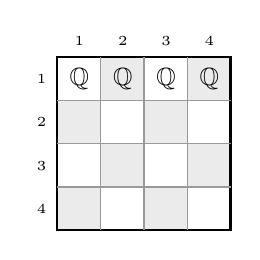
\begin{tikzpicture}
\fill[white] (0.00,0.00) rectangle +(0.55,-0.55);
\fill[black!8] (0.00,-0.55) rectangle +(0.55,-0.55);
\fill[white] (0.00,-1.10) rectangle +(0.55,-0.55);
\fill[black!8] (0.00,-1.65) rectangle +(0.55,-0.55);
\fill[black!8] (0.55,0.00) rectangle +(0.55,-0.55);
\fill[white] (0.55,-0.55) rectangle +(0.55,-0.55);
\fill[black!8] (0.55,-1.10) rectangle +(0.55,-0.55);
\fill[white] (0.55,-1.65) rectangle +(0.55,-0.55);
\fill[white] (1.10,0.00) rectangle +(0.55,-0.55);
\fill[black!8] (1.10,-0.55) rectangle +(0.55,-0.55);
\fill[white] (1.10,-1.10) rectangle +(0.55,-0.55);
\fill[black!8] (1.10,-1.65) rectangle +(0.55,-0.55);
\fill[black!8] (1.65,0.00) rectangle +(0.55,-0.55);
\fill[white] (1.65,-0.55) rectangle +(0.55,-0.55);
\fill[black!8] (1.65,-1.10) rectangle +(0.55,-0.55);
\fill[white] (1.65,-1.65) rectangle +(0.55,-0.55);
\draw[thick] (0,0) rectangle (2.20,-2.20);
\draw[black!40] (0.55,0) -- (0.55,-2.20);
\draw[black!40] (0,-0.55) -- (2.20,-0.55);
\draw[black!40] (1.10,0) -- (1.10,-2.20);
\draw[black!40] (0,-1.10) -- (2.20,-1.10);
\draw[black!40] (1.65,0) -- (1.65,-2.20);
\draw[black!40] (0,-1.65) -- (2.20,-1.65);
\node[font=\small\bfseries] at (0.28,-0.28) {$\mathbb{Q}$};
\node[font=\small\bfseries] at (0.83,-0.28) {$\mathbb{Q}$};
\node[font=\small\bfseries] at (1.38,-0.28) {$\mathbb{Q}$};
\node[font=\small\bfseries] at (1.93,-0.28) {$\mathbb{Q}$};
\node[font=\tiny] at (0.28,0.20) {1};
\node[font=\tiny] at (0.83,0.20) {2};
\node[font=\tiny] at (1.38,0.20) {3};
\node[font=\tiny] at (1.93,0.20) {4};
\node[font=\tiny] at (-0.20,-0.28) {1};
\node[font=\tiny] at (-0.20,-0.83) {2};
\node[font=\tiny] at (-0.20,-1.38) {3};
\node[font=\tiny] at (-0.20,-1.93) {4};
\end{tikzpicture}
\end{adjustbox}
\end{center}
\subq{(a)}How many states are there in total? How many successors does each state have? Explain.
\begin{solbox}
$4^4=\mathbf{256}$ states (each queen in any row of its column); $4\times3=\mathbf{12}$ successors.
\end{solbox}
\subq{(b)}What is $h(S)$? Explain.
\begin{solbox}
All four queens share row 1: every pair attacks, $h(S)=\binom42=\mathbf{6}$.
\end{solbox}
\subq{(c)}Apply steepest-descent hill climbing from $S$. At every step write the $h$ value of each of the 12 successors on the board (in the square the queen would move to) and choose the best one (ties: left-most column, then top row). Stop at a solution or when no successor is better.
\begin{solbox}
Numbers = $h$ after moving the queen of that column to that square; red = chosen move.\par\begin{center}\begin{minipage}[t]{0.32\linewidth}\centering 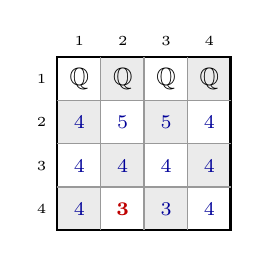
\begin{tikzpicture}
\fill[white] (0.00,0.00) rectangle +(0.55,-0.55);
\fill[black!8] (0.00,-0.55) rectangle +(0.55,-0.55);
\fill[white] (0.00,-1.10) rectangle +(0.55,-0.55);
\fill[black!8] (0.00,-1.65) rectangle +(0.55,-0.55);
\fill[black!8] (0.55,0.00) rectangle +(0.55,-0.55);
\fill[white] (0.55,-0.55) rectangle +(0.55,-0.55);
\fill[black!8] (0.55,-1.10) rectangle +(0.55,-0.55);
\fill[white] (0.55,-1.65) rectangle +(0.55,-0.55);
\fill[white] (1.10,0.00) rectangle +(0.55,-0.55);
\fill[black!8] (1.10,-0.55) rectangle +(0.55,-0.55);
\fill[white] (1.10,-1.10) rectangle +(0.55,-0.55);
\fill[black!8] (1.10,-1.65) rectangle +(0.55,-0.55);
\fill[black!8] (1.65,0.00) rectangle +(0.55,-0.55);
\fill[white] (1.65,-0.55) rectangle +(0.55,-0.55);
\fill[black!8] (1.65,-1.10) rectangle +(0.55,-0.55);
\fill[white] (1.65,-1.65) rectangle +(0.55,-0.55);
\draw[thick] (0,0) rectangle (2.20,-2.20);
\draw[black!40] (0.55,0) -- (0.55,-2.20);
\draw[black!40] (0,-0.55) -- (2.20,-0.55);
\draw[black!40] (1.10,0) -- (1.10,-2.20);
\draw[black!40] (0,-1.10) -- (2.20,-1.10);
\draw[black!40] (1.65,0) -- (1.65,-2.20);
\draw[black!40] (0,-1.65) -- (2.20,-1.65);
\node[font=\small\bfseries] at (0.28,-0.28) {$\mathbb{Q}$};
\node[font=\small\bfseries] at (0.83,-0.28) {$\mathbb{Q}$};
\node[font=\small\bfseries] at (1.38,-0.28) {$\mathbb{Q}$};
\node[font=\small\bfseries] at (1.93,-0.28) {$\mathbb{Q}$};
\node[font=\scriptsize, text=blue!60!black] at (0.28,-0.83) {4};
\node[font=\scriptsize, text=blue!60!black] at (0.83,-0.83) {5};
\node[font=\scriptsize, text=blue!60!black] at (1.38,-0.83) {5};
\node[font=\scriptsize, text=blue!60!black] at (1.93,-0.83) {4};
\node[font=\scriptsize, text=blue!60!black] at (0.28,-1.38) {4};
\node[font=\scriptsize, text=blue!60!black] at (0.83,-1.38) {4};
\node[font=\scriptsize, text=blue!60!black] at (1.38,-1.38) {4};
\node[font=\scriptsize, text=blue!60!black] at (1.93,-1.38) {4};
\node[font=\scriptsize, text=blue!60!black] at (0.28,-1.93) {4};
\node[font=\scriptsize\bfseries, text=red!75!black] at (0.83,-1.93) {3};
\node[font=\scriptsize, text=blue!60!black] at (1.38,-1.93) {3};
\node[font=\scriptsize, text=blue!60!black] at (1.93,-1.93) {4};
\node[font=\tiny] at (0.28,0.20) {1};
\node[font=\tiny] at (0.83,0.20) {2};
\node[font=\tiny] at (1.38,0.20) {3};
\node[font=\tiny] at (1.93,0.20) {4};
\node[font=\tiny] at (-0.20,-0.28) {1};
\node[font=\tiny] at (-0.20,-0.83) {2};
\node[font=\tiny] at (-0.20,-1.38) {3};
\node[font=\tiny] at (-0.20,-1.93) {4};
\end{tikzpicture}\\ \small state $(1,1,1,1)$, $h=6$\end{minipage}\hfill \begin{minipage}[t]{0.32\linewidth}\centering 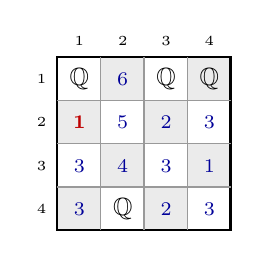
\begin{tikzpicture}
\fill[white] (0.00,0.00) rectangle +(0.55,-0.55);
\fill[black!8] (0.00,-0.55) rectangle +(0.55,-0.55);
\fill[white] (0.00,-1.10) rectangle +(0.55,-0.55);
\fill[black!8] (0.00,-1.65) rectangle +(0.55,-0.55);
\fill[black!8] (0.55,0.00) rectangle +(0.55,-0.55);
\fill[white] (0.55,-0.55) rectangle +(0.55,-0.55);
\fill[black!8] (0.55,-1.10) rectangle +(0.55,-0.55);
\fill[white] (0.55,-1.65) rectangle +(0.55,-0.55);
\fill[white] (1.10,0.00) rectangle +(0.55,-0.55);
\fill[black!8] (1.10,-0.55) rectangle +(0.55,-0.55);
\fill[white] (1.10,-1.10) rectangle +(0.55,-0.55);
\fill[black!8] (1.10,-1.65) rectangle +(0.55,-0.55);
\fill[black!8] (1.65,0.00) rectangle +(0.55,-0.55);
\fill[white] (1.65,-0.55) rectangle +(0.55,-0.55);
\fill[black!8] (1.65,-1.10) rectangle +(0.55,-0.55);
\fill[white] (1.65,-1.65) rectangle +(0.55,-0.55);
\draw[thick] (0,0) rectangle (2.20,-2.20);
\draw[black!40] (0.55,0) -- (0.55,-2.20);
\draw[black!40] (0,-0.55) -- (2.20,-0.55);
\draw[black!40] (1.10,0) -- (1.10,-2.20);
\draw[black!40] (0,-1.10) -- (2.20,-1.10);
\draw[black!40] (1.65,0) -- (1.65,-2.20);
\draw[black!40] (0,-1.65) -- (2.20,-1.65);
\node[font=\small\bfseries] at (0.28,-0.28) {$\mathbb{Q}$};
\node[font=\small\bfseries] at (0.83,-1.93) {$\mathbb{Q}$};
\node[font=\small\bfseries] at (1.38,-0.28) {$\mathbb{Q}$};
\node[font=\small\bfseries] at (1.93,-0.28) {$\mathbb{Q}$};
\node[font=\scriptsize, text=blue!60!black] at (0.83,-0.28) {6};
\node[font=\scriptsize\bfseries, text=red!75!black] at (0.28,-0.83) {1};
\node[font=\scriptsize, text=blue!60!black] at (0.83,-0.83) {5};
\node[font=\scriptsize, text=blue!60!black] at (1.38,-0.83) {2};
\node[font=\scriptsize, text=blue!60!black] at (1.93,-0.83) {3};
\node[font=\scriptsize, text=blue!60!black] at (0.28,-1.38) {3};
\node[font=\scriptsize, text=blue!60!black] at (0.83,-1.38) {4};
\node[font=\scriptsize, text=blue!60!black] at (1.38,-1.38) {3};
\node[font=\scriptsize, text=blue!60!black] at (1.93,-1.38) {1};
\node[font=\scriptsize, text=blue!60!black] at (0.28,-1.93) {3};
\node[font=\scriptsize, text=blue!60!black] at (1.38,-1.93) {2};
\node[font=\scriptsize, text=blue!60!black] at (1.93,-1.93) {3};
\node[font=\tiny] at (0.28,0.20) {1};
\node[font=\tiny] at (0.83,0.20) {2};
\node[font=\tiny] at (1.38,0.20) {3};
\node[font=\tiny] at (1.93,0.20) {4};
\node[font=\tiny] at (-0.20,-0.28) {1};
\node[font=\tiny] at (-0.20,-0.83) {2};
\node[font=\tiny] at (-0.20,-1.38) {3};
\node[font=\tiny] at (-0.20,-1.93) {4};
\end{tikzpicture}\\ \small state $(1,4,1,1)$, $h=3$\end{minipage}\hfill \begin{minipage}[t]{0.32\linewidth}\centering 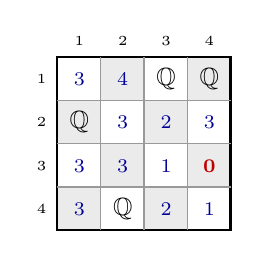
\begin{tikzpicture}
\fill[white] (0.00,0.00) rectangle +(0.55,-0.55);
\fill[black!8] (0.00,-0.55) rectangle +(0.55,-0.55);
\fill[white] (0.00,-1.10) rectangle +(0.55,-0.55);
\fill[black!8] (0.00,-1.65) rectangle +(0.55,-0.55);
\fill[black!8] (0.55,0.00) rectangle +(0.55,-0.55);
\fill[white] (0.55,-0.55) rectangle +(0.55,-0.55);
\fill[black!8] (0.55,-1.10) rectangle +(0.55,-0.55);
\fill[white] (0.55,-1.65) rectangle +(0.55,-0.55);
\fill[white] (1.10,0.00) rectangle +(0.55,-0.55);
\fill[black!8] (1.10,-0.55) rectangle +(0.55,-0.55);
\fill[white] (1.10,-1.10) rectangle +(0.55,-0.55);
\fill[black!8] (1.10,-1.65) rectangle +(0.55,-0.55);
\fill[black!8] (1.65,0.00) rectangle +(0.55,-0.55);
\fill[white] (1.65,-0.55) rectangle +(0.55,-0.55);
\fill[black!8] (1.65,-1.10) rectangle +(0.55,-0.55);
\fill[white] (1.65,-1.65) rectangle +(0.55,-0.55);
\draw[thick] (0,0) rectangle (2.20,-2.20);
\draw[black!40] (0.55,0) -- (0.55,-2.20);
\draw[black!40] (0,-0.55) -- (2.20,-0.55);
\draw[black!40] (1.10,0) -- (1.10,-2.20);
\draw[black!40] (0,-1.10) -- (2.20,-1.10);
\draw[black!40] (1.65,0) -- (1.65,-2.20);
\draw[black!40] (0,-1.65) -- (2.20,-1.65);
\node[font=\small\bfseries] at (0.28,-0.83) {$\mathbb{Q}$};
\node[font=\small\bfseries] at (0.83,-1.93) {$\mathbb{Q}$};
\node[font=\small\bfseries] at (1.38,-0.28) {$\mathbb{Q}$};
\node[font=\small\bfseries] at (1.93,-0.28) {$\mathbb{Q}$};
\node[font=\scriptsize, text=blue!60!black] at (0.28,-0.28) {3};
\node[font=\scriptsize, text=blue!60!black] at (0.83,-0.28) {4};
\node[font=\scriptsize, text=blue!60!black] at (0.83,-0.83) {3};
\node[font=\scriptsize, text=blue!60!black] at (1.38,-0.83) {2};
\node[font=\scriptsize, text=blue!60!black] at (1.93,-0.83) {3};
\node[font=\scriptsize, text=blue!60!black] at (0.28,-1.38) {3};
\node[font=\scriptsize, text=blue!60!black] at (0.83,-1.38) {3};
\node[font=\scriptsize, text=blue!60!black] at (1.38,-1.38) {1};
\node[font=\scriptsize\bfseries, text=red!75!black] at (1.93,-1.38) {0};
\node[font=\scriptsize, text=blue!60!black] at (0.28,-1.93) {3};
\node[font=\scriptsize, text=blue!60!black] at (1.38,-1.93) {2};
\node[font=\scriptsize, text=blue!60!black] at (1.93,-1.93) {1};
\node[font=\tiny] at (0.28,0.20) {1};
\node[font=\tiny] at (0.83,0.20) {2};
\node[font=\tiny] at (1.38,0.20) {3};
\node[font=\tiny] at (1.93,0.20) {4};
\node[font=\tiny] at (-0.20,-0.28) {1};
\node[font=\tiny] at (-0.20,-0.83) {2};
\node[font=\tiny] at (-0.20,-1.38) {3};
\node[font=\tiny] at (-0.20,-1.93) {4};
\end{tikzpicture}\\ \small state $(2,4,1,1)$, $h=1$\end{minipage}\end{center}Level 3: state $(2,4,1,3)$ with $h=0$ --- \textbf{solved}. Hill climbing reaches a solution in 3 moves here (from other states, e.g.\ $(4,3,2,1)$, it gets stuck at $h=1$ without sideways moves).
\end{solbox}
\question{4}Consider the following 4-ply game tree (MAX at the root, children visited left to right).\begin{center}
\begin{adjustbox}{max width=\linewidth}
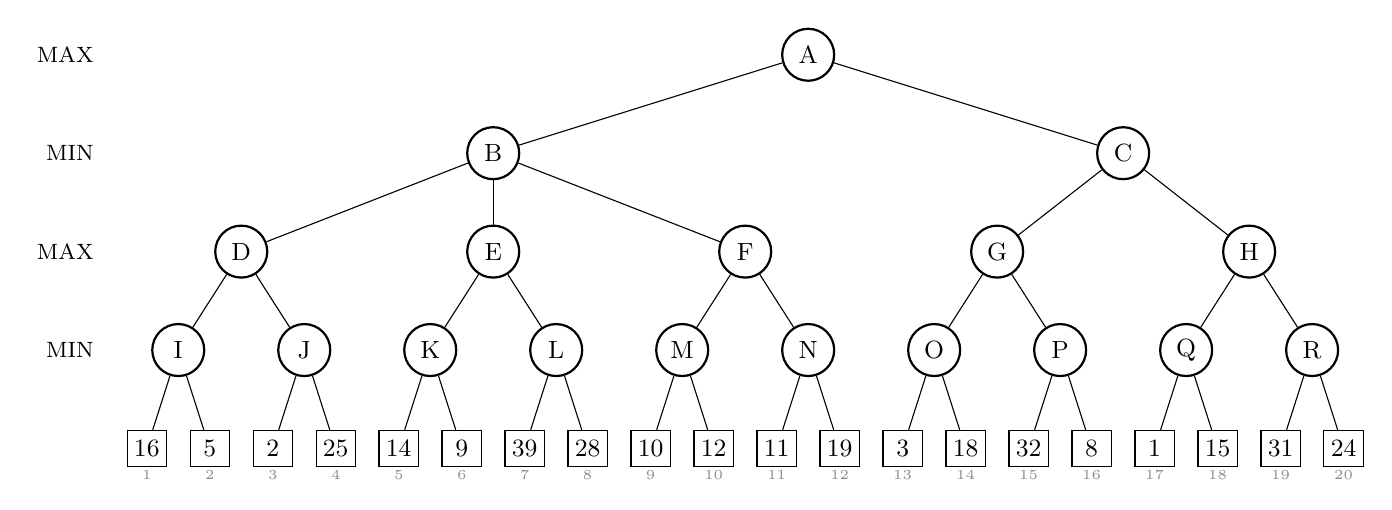
\begin{tikzpicture}[scale=1.0, every node/.style={transform shape}, gc/.style={draw, thick, circle, minimum size=6.6mm, inner sep=0pt, font=\small}, gl/.style={draw, rectangle, minimum width=5mm, minimum height=4.6mm, inner sep=1pt, font=\small}, gx/.style={draw=black!25, text=black!35}, val/.style={font=\footnotesize\bfseries, text=red!80!black, inner sep=1pt}]
\node[font=\footnotesize, anchor=east] at (-0.55,0.00) {MAX};
\node[font=\footnotesize, anchor=east] at (-0.55,-1.25) {MIN};
\node[font=\footnotesize, anchor=east] at (-0.55,-2.50) {MAX};
\node[font=\footnotesize, anchor=east] at (-0.55,-3.75) {MIN};
\node[gc] (n37) at (8.400,0.000) {A};
\node[gc] (n21) at (4.400,-1.250) {B};
\node[gc] (n6) at (1.200,-2.500) {D};
\node[gc] (n2) at (0.400,-3.750) {I};
\node[gl, label={[font=\tiny, text=black!45, inner sep=1pt]below:1}] (n0) at (0.000,-5.000) {16};
\node[gl, label={[font=\tiny, text=black!45, inner sep=1pt]below:2}] (n1) at (0.800,-5.000) {5};
\node[gc] (n5) at (2.000,-3.750) {J};
\node[gl, label={[font=\tiny, text=black!45, inner sep=1pt]below:3}] (n3) at (1.600,-5.000) {2};
\node[gl, label={[font=\tiny, text=black!45, inner sep=1pt]below:4}] (n4) at (2.400,-5.000) {25};
\node[gc] (n13) at (4.400,-2.500) {E};
\node[gc] (n9) at (3.600,-3.750) {K};
\node[gl, label={[font=\tiny, text=black!45, inner sep=1pt]below:5}] (n7) at (3.200,-5.000) {14};
\node[gl, label={[font=\tiny, text=black!45, inner sep=1pt]below:6}] (n8) at (4.000,-5.000) {9};
\node[gc] (n12) at (5.200,-3.750) {L};
\node[gl, label={[font=\tiny, text=black!45, inner sep=1pt]below:7}] (n10) at (4.800,-5.000) {39};
\node[gl, label={[font=\tiny, text=black!45, inner sep=1pt]below:8}] (n11) at (5.600,-5.000) {28};
\node[gc] (n20) at (7.600,-2.500) {F};
\node[gc] (n16) at (6.800,-3.750) {M};
\node[gl, label={[font=\tiny, text=black!45, inner sep=1pt]below:9}] (n14) at (6.400,-5.000) {10};
\node[gl, label={[font=\tiny, text=black!45, inner sep=1pt]below:10}] (n15) at (7.200,-5.000) {12};
\node[gc] (n19) at (8.400,-3.750) {N};
\node[gl, label={[font=\tiny, text=black!45, inner sep=1pt]below:11}] (n17) at (8.000,-5.000) {11};
\node[gl, label={[font=\tiny, text=black!45, inner sep=1pt]below:12}] (n18) at (8.800,-5.000) {19};
\node[gc] (n36) at (12.400,-1.250) {C};
\node[gc] (n28) at (10.800,-2.500) {G};
\node[gc] (n24) at (10.000,-3.750) {O};
\node[gl, label={[font=\tiny, text=black!45, inner sep=1pt]below:13}] (n22) at (9.600,-5.000) {3};
\node[gl, label={[font=\tiny, text=black!45, inner sep=1pt]below:14}] (n23) at (10.400,-5.000) {18};
\node[gc] (n27) at (11.600,-3.750) {P};
\node[gl, label={[font=\tiny, text=black!45, inner sep=1pt]below:15}] (n25) at (11.200,-5.000) {32};
\node[gl, label={[font=\tiny, text=black!45, inner sep=1pt]below:16}] (n26) at (12.000,-5.000) {8};
\node[gc] (n35) at (14.000,-2.500) {H};
\node[gc] (n31) at (13.200,-3.750) {Q};
\node[gl, label={[font=\tiny, text=black!45, inner sep=1pt]below:17}] (n29) at (12.800,-5.000) {1};
\node[gl, label={[font=\tiny, text=black!45, inner sep=1pt]below:18}] (n30) at (13.600,-5.000) {15};
\node[gc] (n34) at (14.800,-3.750) {R};
\node[gl, label={[font=\tiny, text=black!45, inner sep=1pt]below:19}] (n32) at (14.400,-5.000) {31};
\node[gl, label={[font=\tiny, text=black!45, inner sep=1pt]below:20}] (n33) at (15.200,-5.000) {24};
\draw (n37) -- (n21);
\draw (n37) -- (n36);
\draw (n21) -- (n6);
\draw (n21) -- (n13);
\draw (n21) -- (n20);
\draw (n6) -- (n2);
\draw (n6) -- (n5);
\draw (n2) -- (n0);
\draw (n2) -- (n1);
\draw (n5) -- (n3);
\draw (n5) -- (n4);
\draw (n13) -- (n9);
\draw (n13) -- (n12);
\draw (n9) -- (n7);
\draw (n9) -- (n8);
\draw (n12) -- (n10);
\draw (n12) -- (n11);
\draw (n20) -- (n16);
\draw (n20) -- (n19);
\draw (n16) -- (n14);
\draw (n16) -- (n15);
\draw (n19) -- (n17);
\draw (n19) -- (n18);
\draw (n36) -- (n28);
\draw (n36) -- (n35);
\draw (n28) -- (n24);
\draw (n28) -- (n27);
\draw (n24) -- (n22);
\draw (n24) -- (n23);
\draw (n27) -- (n25);
\draw (n27) -- (n26);
\draw (n35) -- (n31);
\draw (n35) -- (n34);
\draw (n31) -- (n29);
\draw (n31) -- (n30);
\draw (n34) -- (n32);
\draw (n34) -- (n33);
\end{tikzpicture}
\end{adjustbox}
\end{center}
\subq{(a)}Compute the final backed-up value of every node using the minimax algorithm (no alpha-beta pruning at this step). Which move should MAX make at the root?
\begin{solbox}
\begin{center}\small \begin{tabular}{|l|c|c|c|c|c|c|c|c|c|}\hline
\textbf{Node} & \textbf{A} & \textbf{B} & \textbf{C} & \textbf{D} & \textbf{E} & \textbf{F} & \textbf{G} & \textbf{H} & \textbf{I}\\ \hline
Minimax & \textcolor{blue!60!black}{8} & \textcolor{blue!60!black}{5} & \textcolor{blue!60!black}{8} & \textcolor{blue!60!black}{5} & \textcolor{blue!60!black}{28} & \textcolor{blue!60!black}{11} & \textcolor{blue!60!black}{8} & \textcolor{blue!60!black}{24} & \textcolor{blue!60!black}{5}\\[1.5mm] \hline
\end{tabular}\\[2mm]\begin{tabular}{|l|c|c|c|c|c|c|c|c|c|}\hline
\textbf{Node} & \textbf{J} & \textbf{K} & \textbf{L} & \textbf{M} & \textbf{N} & \textbf{O} & \textbf{P} & \textbf{Q} & \textbf{R}\\ \hline
Minimax & \textcolor{blue!60!black}{2} & \textcolor{blue!60!black}{9} & \textcolor{blue!60!black}{28} & \textcolor{blue!60!black}{10} & \textcolor{blue!60!black}{11} & \textcolor{blue!60!black}{3} & \textcolor{blue!60!black}{8} & \textcolor{blue!60!black}{1} & \textcolor{blue!60!black}{24}\\[1.5mm] \hline
\end{tabular}\end{center}\begin{center}
\begin{adjustbox}{max width=\linewidth}
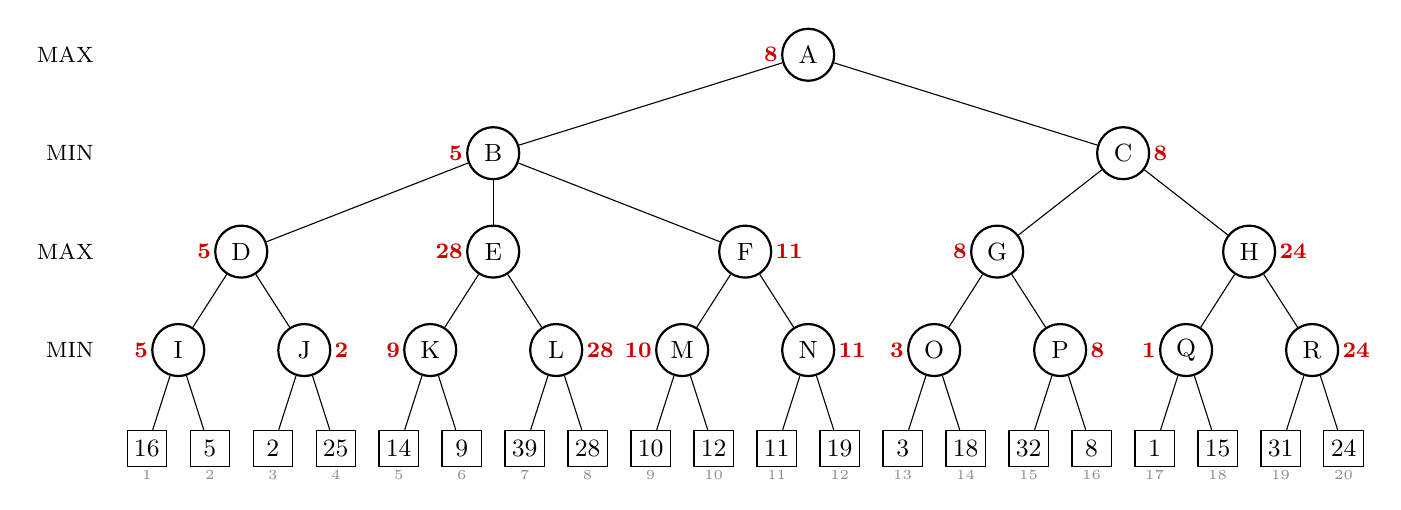
\begin{tikzpicture}[scale=1.0, every node/.style={transform shape}, gc/.style={draw, thick, circle, minimum size=6.6mm, inner sep=0pt, font=\small}, gl/.style={draw, rectangle, minimum width=5mm, minimum height=4.6mm, inner sep=1pt, font=\small}, gx/.style={draw=black!25, text=black!35}, val/.style={font=\footnotesize\bfseries, text=red!80!black, inner sep=1pt}]
\node[font=\footnotesize, anchor=east] at (-0.55,0.00) {MAX};
\node[font=\footnotesize, anchor=east] at (-0.55,-1.25) {MIN};
\node[font=\footnotesize, anchor=east] at (-0.55,-2.50) {MAX};
\node[font=\footnotesize, anchor=east] at (-0.55,-3.75) {MIN};
\node[gc, label={[val]left:8}] (n37) at (8.400,0.000) {A};
\node[gc, label={[val]left:5}] (n21) at (4.400,-1.250) {B};
\node[gc, label={[val]left:5}] (n6) at (1.200,-2.500) {D};
\node[gc, label={[val]left:5}] (n2) at (0.400,-3.750) {I};
\node[gl, label={[font=\tiny, text=black!45, inner sep=1pt]below:1}] (n0) at (0.000,-5.000) {16};
\node[gl, label={[font=\tiny, text=black!45, inner sep=1pt]below:2}] (n1) at (0.800,-5.000) {5};
\node[gc, label={[val]right:2}] (n5) at (2.000,-3.750) {J};
\node[gl, label={[font=\tiny, text=black!45, inner sep=1pt]below:3}] (n3) at (1.600,-5.000) {2};
\node[gl, label={[font=\tiny, text=black!45, inner sep=1pt]below:4}] (n4) at (2.400,-5.000) {25};
\node[gc, label={[val]left:28}] (n13) at (4.400,-2.500) {E};
\node[gc, label={[val]left:9}] (n9) at (3.600,-3.750) {K};
\node[gl, label={[font=\tiny, text=black!45, inner sep=1pt]below:5}] (n7) at (3.200,-5.000) {14};
\node[gl, label={[font=\tiny, text=black!45, inner sep=1pt]below:6}] (n8) at (4.000,-5.000) {9};
\node[gc, label={[val]right:28}] (n12) at (5.200,-3.750) {L};
\node[gl, label={[font=\tiny, text=black!45, inner sep=1pt]below:7}] (n10) at (4.800,-5.000) {39};
\node[gl, label={[font=\tiny, text=black!45, inner sep=1pt]below:8}] (n11) at (5.600,-5.000) {28};
\node[gc, label={[val]right:11}] (n20) at (7.600,-2.500) {F};
\node[gc, label={[val]left:10}] (n16) at (6.800,-3.750) {M};
\node[gl, label={[font=\tiny, text=black!45, inner sep=1pt]below:9}] (n14) at (6.400,-5.000) {10};
\node[gl, label={[font=\tiny, text=black!45, inner sep=1pt]below:10}] (n15) at (7.200,-5.000) {12};
\node[gc, label={[val]right:11}] (n19) at (8.400,-3.750) {N};
\node[gl, label={[font=\tiny, text=black!45, inner sep=1pt]below:11}] (n17) at (8.000,-5.000) {11};
\node[gl, label={[font=\tiny, text=black!45, inner sep=1pt]below:12}] (n18) at (8.800,-5.000) {19};
\node[gc, label={[val]right:8}] (n36) at (12.400,-1.250) {C};
\node[gc, label={[val]left:8}] (n28) at (10.800,-2.500) {G};
\node[gc, label={[val]left:3}] (n24) at (10.000,-3.750) {O};
\node[gl, label={[font=\tiny, text=black!45, inner sep=1pt]below:13}] (n22) at (9.600,-5.000) {3};
\node[gl, label={[font=\tiny, text=black!45, inner sep=1pt]below:14}] (n23) at (10.400,-5.000) {18};
\node[gc, label={[val]right:8}] (n27) at (11.600,-3.750) {P};
\node[gl, label={[font=\tiny, text=black!45, inner sep=1pt]below:15}] (n25) at (11.200,-5.000) {32};
\node[gl, label={[font=\tiny, text=black!45, inner sep=1pt]below:16}] (n26) at (12.000,-5.000) {8};
\node[gc, label={[val]right:24}] (n35) at (14.000,-2.500) {H};
\node[gc, label={[val]left:1}] (n31) at (13.200,-3.750) {Q};
\node[gl, label={[font=\tiny, text=black!45, inner sep=1pt]below:17}] (n29) at (12.800,-5.000) {1};
\node[gl, label={[font=\tiny, text=black!45, inner sep=1pt]below:18}] (n30) at (13.600,-5.000) {15};
\node[gc, label={[val]right:24}] (n34) at (14.800,-3.750) {R};
\node[gl, label={[font=\tiny, text=black!45, inner sep=1pt]below:19}] (n32) at (14.400,-5.000) {31};
\node[gl, label={[font=\tiny, text=black!45, inner sep=1pt]below:20}] (n33) at (15.200,-5.000) {24};
\draw (n37) -- (n21);
\draw (n37) -- (n36);
\draw (n21) -- (n6);
\draw (n21) -- (n13);
\draw (n21) -- (n20);
\draw (n6) -- (n2);
\draw (n6) -- (n5);
\draw (n2) -- (n0);
\draw (n2) -- (n1);
\draw (n5) -- (n3);
\draw (n5) -- (n4);
\draw (n13) -- (n9);
\draw (n13) -- (n12);
\draw (n9) -- (n7);
\draw (n9) -- (n8);
\draw (n12) -- (n10);
\draw (n12) -- (n11);
\draw (n20) -- (n16);
\draw (n20) -- (n19);
\draw (n16) -- (n14);
\draw (n16) -- (n15);
\draw (n19) -- (n17);
\draw (n19) -- (n18);
\draw (n36) -- (n28);
\draw (n36) -- (n35);
\draw (n28) -- (n24);
\draw (n28) -- (n27);
\draw (n24) -- (n22);
\draw (n24) -- (n23);
\draw (n27) -- (n25);
\draw (n27) -- (n26);
\draw (n35) -- (n31);
\draw (n35) -- (n34);
\draw (n31) -- (n29);
\draw (n31) -- (n30);
\draw (n34) -- (n32);
\draw (n34) -- (n33);
\end{tikzpicture}
\end{adjustbox}
\end{center}Root value $=8$; MAX moves to \textbf{C}.
\end{solbox}
\subq{(b)}Run alpha-beta pruning (children visited left to right). Give the value computed at every node (mark \textbf{X} if the node is never visited), cross out the pruned branches on the tree and briefly explain each case.
\begin{solbox}
\begin{center}\small \begin{tabular}{|l|c|c|c|c|c|c|c|c|c|}\hline
\textbf{Node} & \textbf{A} & \textbf{B} & \textbf{C} & \textbf{D} & \textbf{E} & \textbf{F} & \textbf{G} & \textbf{H} & \textbf{I}\\ \hline
$\alpha$-$\beta$ & \textcolor{blue!60!black}{$8$} & \textcolor{blue!60!black}{$5$} & \textcolor{blue!60!black}{$8$} & \textcolor{blue!60!black}{$5$} & \textcolor{blue!60!black}{$\ge 9$} & \textcolor{blue!60!black}{$\ge 10$} & \textcolor{blue!60!black}{$8$} & \textcolor{blue!60!black}{$24$} & \textcolor{blue!60!black}{$5$}\\[1.5mm] \hline
\end{tabular}\\[2mm]\begin{tabular}{|l|c|c|c|c|c|c|c|c|c|}\hline
\textbf{Node} & \textbf{J} & \textbf{K} & \textbf{L} & \textbf{M} & \textbf{N} & \textbf{O} & \textbf{P} & \textbf{Q} & \textbf{R}\\ \hline
$\alpha$-$\beta$ & \textcolor{blue!60!black}{$\le 2$} & \textcolor{blue!60!black}{$9$} & \textcolor{red!70!black}{\textbf{X}} & \textcolor{blue!60!black}{$10$} & \textcolor{red!70!black}{\textbf{X}} & \textcolor{blue!60!black}{$\le 3$} & \textcolor{blue!60!black}{$8$} & \textcolor{blue!60!black}{$\le 1$} & \textcolor{blue!60!black}{$24$}\\[1.5mm] \hline
\end{tabular}\end{center}($\le v$ / $\ge v$: the node was cut off, so only this bound is known; writing the returned number $v$ is also accepted.)\begin{center}
\begin{adjustbox}{max width=\linewidth}
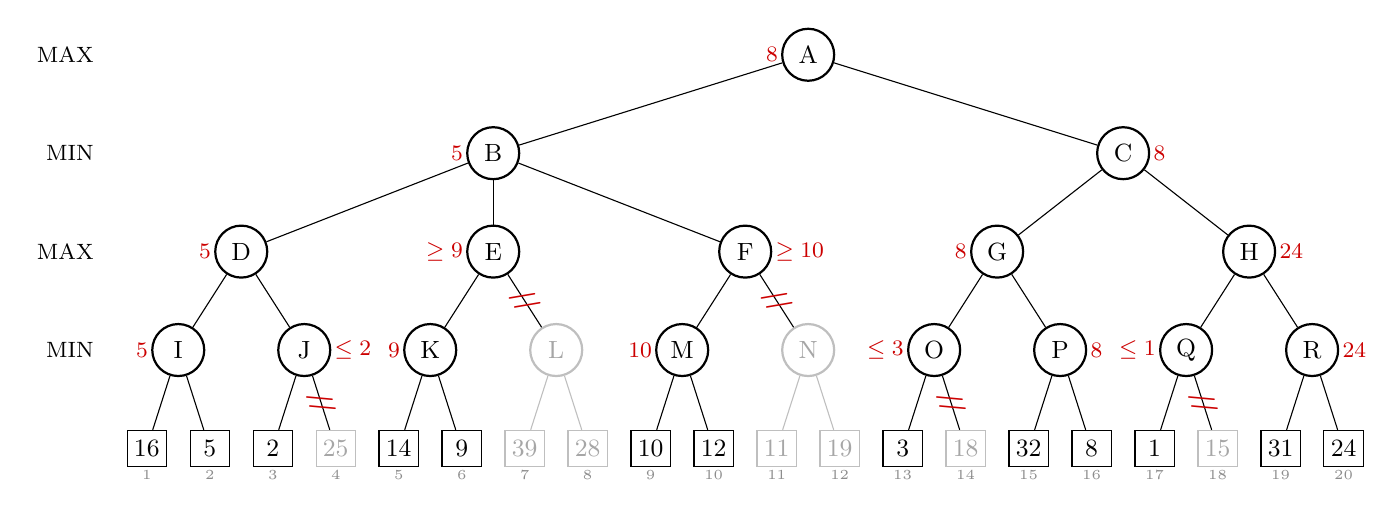
\begin{tikzpicture}[scale=1.0, every node/.style={transform shape}, gc/.style={draw, thick, circle, minimum size=6.6mm, inner sep=0pt, font=\small}, gl/.style={draw, rectangle, minimum width=5mm, minimum height=4.6mm, inner sep=1pt, font=\small}, gx/.style={draw=black!25, text=black!35}, val/.style={font=\footnotesize\bfseries, text=red!80!black, inner sep=1pt}]
\node[font=\footnotesize, anchor=east] at (-0.55,0.00) {MAX};
\node[font=\footnotesize, anchor=east] at (-0.55,-1.25) {MIN};
\node[font=\footnotesize, anchor=east] at (-0.55,-2.50) {MAX};
\node[font=\footnotesize, anchor=east] at (-0.55,-3.75) {MIN};
\node[gc, label={[val]left:$8$}] (n37) at (8.400,0.000) {A};
\node[gc, label={[val]left:$5$}] (n21) at (4.400,-1.250) {B};
\node[gc, label={[val]left:$5$}] (n6) at (1.200,-2.500) {D};
\node[gc, label={[val]left:$5$}] (n2) at (0.400,-3.750) {I};
\node[gl, label={[font=\tiny, text=black!45, inner sep=1pt]below:1}] (n0) at (0.000,-5.000) {16};
\node[gl, label={[font=\tiny, text=black!45, inner sep=1pt]below:2}] (n1) at (0.800,-5.000) {5};
\node[gc, label={[val]right:$\le2$}] (n5) at (2.000,-3.750) {J};
\node[gl, label={[font=\tiny, text=black!45, inner sep=1pt]below:3}] (n3) at (1.600,-5.000) {2};
\node[gl, gx, label={[font=\tiny, text=black!45, inner sep=1pt]below:4}] (n4) at (2.400,-5.000) {25};
\node[gc, label={[val]left:$\ge9$}] (n13) at (4.400,-2.500) {E};
\node[gc, label={[val]left:$9$}] (n9) at (3.600,-3.750) {K};
\node[gl, label={[font=\tiny, text=black!45, inner sep=1pt]below:5}] (n7) at (3.200,-5.000) {14};
\node[gl, label={[font=\tiny, text=black!45, inner sep=1pt]below:6}] (n8) at (4.000,-5.000) {9};
\node[gc, gx] (n12) at (5.200,-3.750) {L};
\node[gl, gx, label={[font=\tiny, text=black!45, inner sep=1pt]below:7}] (n10) at (4.800,-5.000) {39};
\node[gl, gx, label={[font=\tiny, text=black!45, inner sep=1pt]below:8}] (n11) at (5.600,-5.000) {28};
\node[gc, label={[val]right:$\ge10$}] (n20) at (7.600,-2.500) {F};
\node[gc, label={[val]left:$10$}] (n16) at (6.800,-3.750) {M};
\node[gl, label={[font=\tiny, text=black!45, inner sep=1pt]below:9}] (n14) at (6.400,-5.000) {10};
\node[gl, label={[font=\tiny, text=black!45, inner sep=1pt]below:10}] (n15) at (7.200,-5.000) {12};
\node[gc, gx] (n19) at (8.400,-3.750) {N};
\node[gl, gx, label={[font=\tiny, text=black!45, inner sep=1pt]below:11}] (n17) at (8.000,-5.000) {11};
\node[gl, gx, label={[font=\tiny, text=black!45, inner sep=1pt]below:12}] (n18) at (8.800,-5.000) {19};
\node[gc, label={[val]right:$8$}] (n36) at (12.400,-1.250) {C};
\node[gc, label={[val]left:$8$}] (n28) at (10.800,-2.500) {G};
\node[gc, label={[val]left:$\le3$}] (n24) at (10.000,-3.750) {O};
\node[gl, label={[font=\tiny, text=black!45, inner sep=1pt]below:13}] (n22) at (9.600,-5.000) {3};
\node[gl, gx, label={[font=\tiny, text=black!45, inner sep=1pt]below:14}] (n23) at (10.400,-5.000) {18};
\node[gc, label={[val]right:$8$}] (n27) at (11.600,-3.750) {P};
\node[gl, label={[font=\tiny, text=black!45, inner sep=1pt]below:15}] (n25) at (11.200,-5.000) {32};
\node[gl, label={[font=\tiny, text=black!45, inner sep=1pt]below:16}] (n26) at (12.000,-5.000) {8};
\node[gc, label={[val]right:$24$}] (n35) at (14.000,-2.500) {H};
\node[gc, label={[val]left:$\le1$}] (n31) at (13.200,-3.750) {Q};
\node[gl, label={[font=\tiny, text=black!45, inner sep=1pt]below:17}] (n29) at (12.800,-5.000) {1};
\node[gl, gx, label={[font=\tiny, text=black!45, inner sep=1pt]below:18}] (n30) at (13.600,-5.000) {15};
\node[gc, label={[val]right:$24$}] (n34) at (14.800,-3.750) {R};
\node[gl, label={[font=\tiny, text=black!45, inner sep=1pt]below:19}] (n32) at (14.400,-5.000) {31};
\node[gl, label={[font=\tiny, text=black!45, inner sep=1pt]below:20}] (n33) at (15.200,-5.000) {24};
\draw (n37) -- (n21);
\draw (n37) -- (n36);
\draw (n21) -- (n6);
\draw (n21) -- (n13);
\draw (n21) -- (n20);
\draw (n6) -- (n2);
\draw (n6) -- (n5);
\draw (n2) -- (n0);
\draw (n2) -- (n1);
\draw (n5) -- (n3);
\draw (n5) -- (n4) node[midway, sloped, text=red!80!black, font=\small\bfseries, inner sep=0pt]{/\!/};
\draw (n13) -- (n9);
\draw (n13) -- (n12) node[midway, sloped, text=red!80!black, font=\small\bfseries, inner sep=0pt]{/\!/};
\draw (n9) -- (n7);
\draw (n9) -- (n8);
\draw[black!25] (n12) -- (n10);
\draw[black!25] (n12) -- (n11);
\draw (n20) -- (n16);
\draw (n20) -- (n19) node[midway, sloped, text=red!80!black, font=\small\bfseries, inner sep=0pt]{/\!/};
\draw (n16) -- (n14);
\draw (n16) -- (n15);
\draw[black!25] (n19) -- (n17);
\draw[black!25] (n19) -- (n18);
\draw (n36) -- (n28);
\draw (n36) -- (n35);
\draw (n28) -- (n24);
\draw (n28) -- (n27);
\draw (n24) -- (n22);
\draw (n24) -- (n23) node[midway, sloped, text=red!80!black, font=\small\bfseries, inner sep=0pt]{/\!/};
\draw (n27) -- (n25);
\draw (n27) -- (n26);
\draw (n35) -- (n31);
\draw (n35) -- (n34);
\draw (n31) -- (n29);
\draw (n31) -- (n30) node[midway, sloped, text=red!80!black, font=\small\bfseries, inner sep=0pt]{/\!/};
\draw (n34) -- (n32);
\draw (n34) -- (n33);
\end{tikzpicture}
\end{adjustbox}
\end{center}$\alpha$ and $\beta$ at every visited node:\begin{center}\small\begin{tabular}{c c c c c}\toprule Node & Type & On entry & When it returns & Value returned\\\midrule A & MAX & $\alpha=-\infty,\ \beta=+\infty$ & $\alpha=8,\ \beta=+\infty$ & $8$ \\
B & MIN & $\alpha=-\infty,\ \beta=+\infty$ & $\alpha=-\infty,\ \beta=5$ & $5$ \\
D & MAX & $\alpha=-\infty,\ \beta=+\infty$ & $\alpha=5,\ \beta=+\infty$ & $5$ \\
I & MIN & $\alpha=-\infty,\ \beta=+\infty$ & $\alpha=-\infty,\ \beta=5$ & $5$ \\
J & MIN & $\alpha=5,\ \beta=+\infty$ & $\alpha=5,\ \beta=2$ & $\le 2$ \\
E & MAX & $\alpha=-\infty,\ \beta=5$ & $\alpha=9,\ \beta=5$ & $\ge 9$ \\
K & MIN & $\alpha=-\infty,\ \beta=5$ & $\alpha=-\infty,\ \beta=5$ & $9$ \\
F & MAX & $\alpha=-\infty,\ \beta=5$ & $\alpha=10,\ \beta=5$ & $\ge 10$ \\
M & MIN & $\alpha=-\infty,\ \beta=5$ & $\alpha=-\infty,\ \beta=5$ & $10$ \\
C & MIN & $\alpha=5,\ \beta=+\infty$ & $\alpha=5,\ \beta=8$ & $8$ \\
G & MAX & $\alpha=5,\ \beta=+\infty$ & $\alpha=8,\ \beta=+\infty$ & $8$ \\
O & MIN & $\alpha=5,\ \beta=+\infty$ & $\alpha=5,\ \beta=3$ & $\le 3$ \\
P & MIN & $\alpha=5,\ \beta=+\infty$ & $\alpha=5,\ \beta=8$ & $8$ \\
H & MAX & $\alpha=5,\ \beta=8$ & $\alpha=24,\ \beta=8$ & $24$ \\
Q & MIN & $\alpha=5,\ \beta=8$ & $\alpha=5,\ \beta=1$ & $\le 1$ \\
R & MIN & $\alpha=5,\ \beta=8$ & $\alpha=5,\ \beta=8$ & $24$ \\\bottomrule\end{tabular}\end{center}\begin{itemize}[leftmargin=1.5em,itemsep=1pt]
\item At MIN node \textbf{J}, after leaf \#3: $v=2 \le \alpha=5$ $\Rightarrow$ prune leaf \#4. (MAX at D already has an alternative worth $\alpha=5$, so it will never let play reach J.)
\item At MAX node \textbf{E}, after child K: $v=9 \ge \beta=5$ $\Rightarrow$ prune L (leaves \#7--\#8). (MIN at B already has an alternative worth $\beta=5$, so it will never let play reach E.)
\item At MAX node \textbf{F}, after child M: $v=10 \ge \beta=5$ $\Rightarrow$ prune N (leaves \#11--\#12). (MIN at B already has an alternative worth $\beta=5$, so it will never let play reach F.)
\item At MIN node \textbf{O}, after leaf \#13: $v=3 \le \alpha=5$ $\Rightarrow$ prune leaf \#14. (MAX at A already has an alternative worth $\alpha=5$, so it will never let play reach O.) \textbf{Deep cut-off}: the bound comes from A, 3 levels above O.
\item At MIN node \textbf{Q}, after leaf \#17: $v=1 \le \alpha=5$ $\Rightarrow$ prune leaf \#18. (MAX at A already has an alternative worth $\alpha=5$, so it will never let play reach Q.) \textbf{Deep cut-off}: the bound comes from A, 3 levels above Q.
\end{itemize}Leaves evaluated: 13 of 20.
\end{solbox}
\subq{(c)}Using the minimax values from (a), and without performing any alpha-beta calculation, rotate the children of each node at every level so that alpha-beta prunes as much as possible. Draw the new tree (keep the node letters).
\begin{solbox}
Best child first for the player to move (MAX: largest value first, MIN: smallest first):\begin{center}
\begin{adjustbox}{max width=\linewidth}
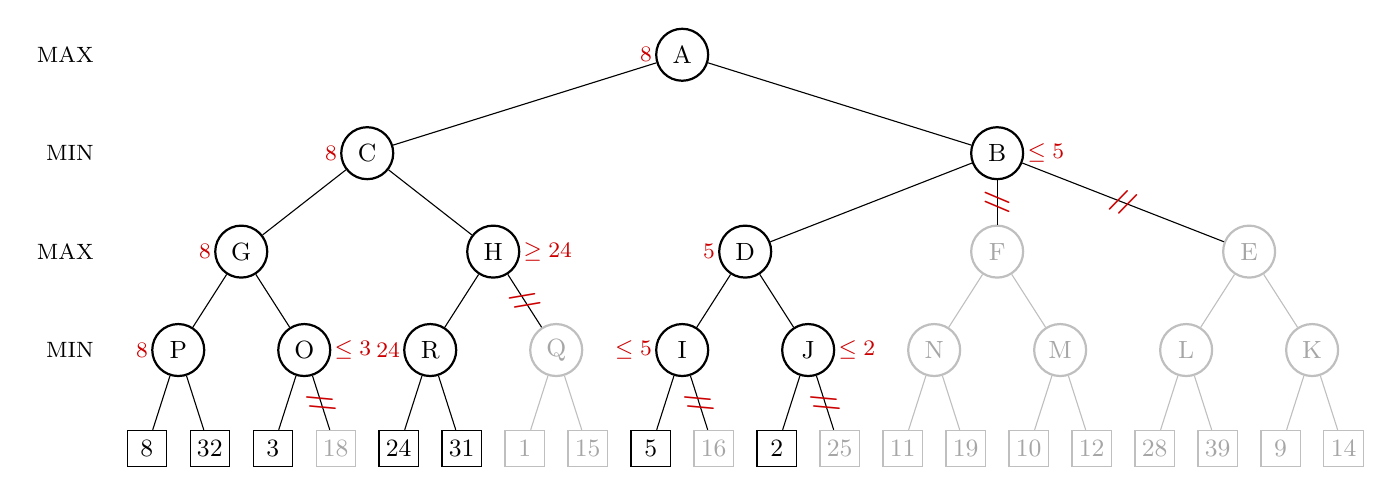
\begin{tikzpicture}[scale=1.0, every node/.style={transform shape}, gc/.style={draw, thick, circle, minimum size=6.6mm, inner sep=0pt, font=\small}, gl/.style={draw, rectangle, minimum width=5mm, minimum height=4.6mm, inner sep=1pt, font=\small}, gx/.style={draw=black!25, text=black!35}, val/.style={font=\footnotesize\bfseries, text=red!80!black, inner sep=1pt}]
\node[font=\footnotesize, anchor=east] at (-0.55,0.00) {MAX};
\node[font=\footnotesize, anchor=east] at (-0.55,-1.25) {MIN};
\node[font=\footnotesize, anchor=east] at (-0.55,-2.50) {MAX};
\node[font=\footnotesize, anchor=east] at (-0.55,-3.75) {MIN};
\node[gc, label={[val]left:$8$}] (n37) at (6.800,0.000) {A};
\node[gc, label={[val]left:$8$}] (n14) at (2.800,-1.250) {C};
\node[gc, label={[val]left:$8$}] (n6) at (1.200,-2.500) {G};
\node[gc, label={[val]left:$8$}] (n2) at (0.400,-3.750) {P};
\node[gl] (n0) at (0.000,-5.000) {8};
\node[gl] (n1) at (0.800,-5.000) {32};
\node[gc, label={[val]right:$\le3$}] (n5) at (2.000,-3.750) {O};
\node[gl] (n3) at (1.600,-5.000) {3};
\node[gl, gx] (n4) at (2.400,-5.000) {18};
\node[gc, label={[val]right:$\ge24$}] (n13) at (4.400,-2.500) {H};
\node[gc, label={[val]left:$24$}] (n9) at (3.600,-3.750) {R};
\node[gl] (n7) at (3.200,-5.000) {24};
\node[gl] (n8) at (4.000,-5.000) {31};
\node[gc, gx] (n12) at (5.200,-3.750) {Q};
\node[gl, gx] (n10) at (4.800,-5.000) {1};
\node[gl, gx] (n11) at (5.600,-5.000) {15};
\node[gc, label={[val]right:$\le5$}] (n36) at (10.800,-1.250) {B};
\node[gc, label={[val]left:$5$}] (n21) at (7.600,-2.500) {D};
\node[gc, label={[val]left:$\le5$}] (n17) at (6.800,-3.750) {I};
\node[gl] (n15) at (6.400,-5.000) {5};
\node[gl, gx] (n16) at (7.200,-5.000) {16};
\node[gc, label={[val]right:$\le2$}] (n20) at (8.400,-3.750) {J};
\node[gl] (n18) at (8.000,-5.000) {2};
\node[gl, gx] (n19) at (8.800,-5.000) {25};
\node[gc, gx] (n28) at (10.800,-2.500) {F};
\node[gc, gx] (n24) at (10.000,-3.750) {N};
\node[gl, gx] (n22) at (9.600,-5.000) {11};
\node[gl, gx] (n23) at (10.400,-5.000) {19};
\node[gc, gx] (n27) at (11.600,-3.750) {M};
\node[gl, gx] (n25) at (11.200,-5.000) {10};
\node[gl, gx] (n26) at (12.000,-5.000) {12};
\node[gc, gx] (n35) at (14.000,-2.500) {E};
\node[gc, gx] (n31) at (13.200,-3.750) {L};
\node[gl, gx] (n29) at (12.800,-5.000) {28};
\node[gl, gx] (n30) at (13.600,-5.000) {39};
\node[gc, gx] (n34) at (14.800,-3.750) {K};
\node[gl, gx] (n32) at (14.400,-5.000) {9};
\node[gl, gx] (n33) at (15.200,-5.000) {14};
\draw (n37) -- (n14);
\draw (n37) -- (n36);
\draw (n14) -- (n6);
\draw (n14) -- (n13);
\draw (n6) -- (n2);
\draw (n6) -- (n5);
\draw (n2) -- (n0);
\draw (n2) -- (n1);
\draw (n5) -- (n3);
\draw (n5) -- (n4) node[midway, sloped, text=red!80!black, font=\small\bfseries, inner sep=0pt]{/\!/};
\draw (n13) -- (n9);
\draw (n13) -- (n12) node[midway, sloped, text=red!80!black, font=\small\bfseries, inner sep=0pt]{/\!/};
\draw (n9) -- (n7);
\draw (n9) -- (n8);
\draw[black!25] (n12) -- (n10);
\draw[black!25] (n12) -- (n11);
\draw (n36) -- (n21);
\draw (n36) -- (n28) node[midway, sloped, text=red!80!black, font=\small\bfseries, inner sep=0pt]{/\!/};
\draw (n36) -- (n35) node[midway, sloped, text=red!80!black, font=\small\bfseries, inner sep=0pt]{/\!/};
\draw (n21) -- (n17);
\draw (n21) -- (n20);
\draw (n17) -- (n15);
\draw (n17) -- (n16) node[midway, sloped, text=red!80!black, font=\small\bfseries, inner sep=0pt]{/\!/};
\draw (n20) -- (n18);
\draw (n20) -- (n19) node[midway, sloped, text=red!80!black, font=\small\bfseries, inner sep=0pt]{/\!/};
\draw[black!25] (n28) -- (n24);
\draw[black!25] (n28) -- (n27);
\draw[black!25] (n24) -- (n22);
\draw[black!25] (n24) -- (n23);
\draw[black!25] (n27) -- (n25);
\draw[black!25] (n27) -- (n26);
\draw[black!25] (n35) -- (n31);
\draw[black!25] (n35) -- (n34);
\draw[black!25] (n31) -- (n29);
\draw[black!25] (n31) -- (n30);
\draw[black!25] (n34) -- (n32);
\draw[black!25] (n34) -- (n33);
\end{tikzpicture}
\end{adjustbox}
\end{center}With this ordering alpha-beta evaluates only \textbf{7} leaves (instead of 13).
\end{solbox}
\question{5}The game tree below contains an unknown integer leaf value $x$. Alpha-beta visits children left to right.\begin{center}
\begin{adjustbox}{max width=\linewidth}
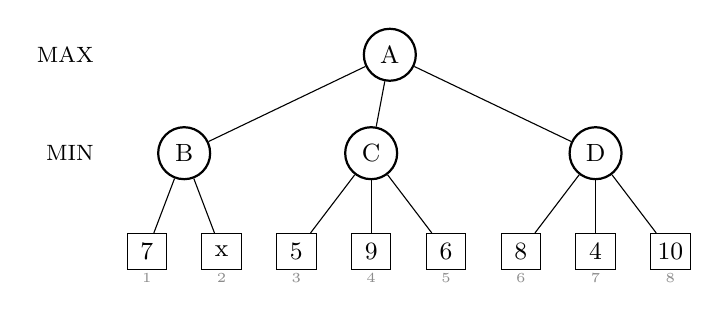
\begin{tikzpicture}[scale=1.0, every node/.style={transform shape}, gc/.style={draw, thick, circle, minimum size=6.6mm, inner sep=0pt, font=\small}, gl/.style={draw, rectangle, minimum width=5mm, minimum height=4.6mm, inner sep=1pt, font=\small}, gx/.style={draw=black!25, text=black!35}, val/.style={font=\footnotesize\bfseries, text=red!80!black, inner sep=1pt}]
\node[font=\footnotesize, anchor=east] at (-0.55,0.00) {MAX};
\node[font=\footnotesize, anchor=east] at (-0.55,-1.25) {MIN};
\node[gc] (n11) at (3.087,0.000) {A};
\node[gc] (n2) at (0.475,-1.250) {B};
\node[gl, label={[font=\tiny, text=black!45, inner sep=1pt]below:1}] (n0) at (0.000,-2.500) {7};
\node[gl, label={[font=\tiny, text=black!45, inner sep=1pt]below:2}] (n1) at (0.950,-2.500) {x};
\node[gc] (n6) at (2.850,-1.250) {C};
\node[gl, label={[font=\tiny, text=black!45, inner sep=1pt]below:3}] (n3) at (1.900,-2.500) {5};
\node[gl, label={[font=\tiny, text=black!45, inner sep=1pt]below:4}] (n4) at (2.850,-2.500) {9};
\node[gl, label={[font=\tiny, text=black!45, inner sep=1pt]below:5}] (n5) at (3.800,-2.500) {6};
\node[gc] (n10) at (5.700,-1.250) {D};
\node[gl, label={[font=\tiny, text=black!45, inner sep=1pt]below:6}] (n7) at (4.750,-2.500) {8};
\node[gl, label={[font=\tiny, text=black!45, inner sep=1pt]below:7}] (n8) at (5.700,-2.500) {4};
\node[gl, label={[font=\tiny, text=black!45, inner sep=1pt]below:8}] (n9) at (6.650,-2.500) {10};
\draw (n11) -- (n2);
\draw (n11) -- (n6);
\draw (n11) -- (n10);
\draw (n2) -- (n0);
\draw (n2) -- (n1);
\draw (n6) -- (n3);
\draw (n6) -- (n4);
\draw (n6) -- (n5);
\draw (n10) -- (n7);
\draw (n10) -- (n8);
\draw (n10) -- (n9);
\end{tikzpicture}
\end{adjustbox}
\end{center}
\subq{(a)}For which values of $x$ are leaves \#4 and \#5 pruned?
\begin{solbox}
After B, $\alpha=\min(7,x)$. C sees leaf \#3 $=5$, so it is cut off iff $5\le\min(7,x)$, i.e.\ $\mathbf{x\ge5}$.
\end{solbox}
\subq{(b)}Is leaf \#8 ever evaluated?
\begin{solbox}
\textbf{Never}: $\alpha\ge5$ when D is entered; after 8 and then 4, $v_D=4\le\alpha$, so leaf \#8 (10) is pruned.
\end{solbox}
\subq{(c)}Give the root value as a function of $x$ and say for which $x$ MAX chooses B.
\begin{solbox}
Root $=\max(\min(7,x),5,4)$: $5$ if $x\le5$; $x$ if $5\le x\le7$; $7$ if $x\ge7$. MAX chooses B iff $x\ge5$ (tie at $x=5$ keeps the left-most child). Checked for $x=0,\dots,12$.
\end{solbox}
\question{6}Consider the expectimax tree below; each chance node has three equally likely outcomes.\begin{center}
\begin{adjustbox}{max width=\linewidth}
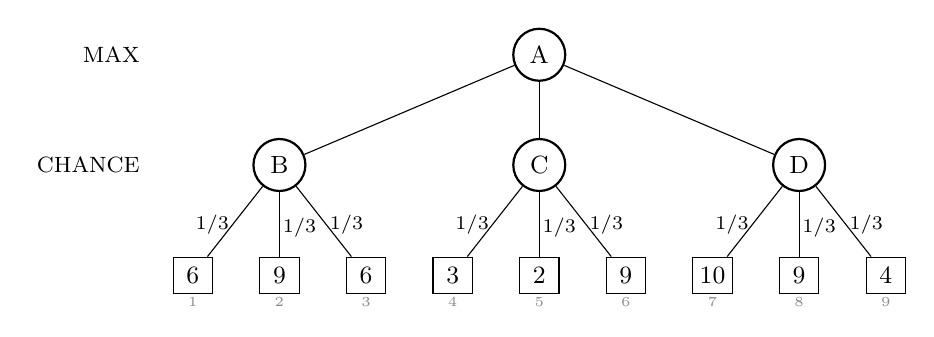
\begin{tikzpicture}[scale=1.0, every node/.style={transform shape}, gc/.style={draw, thick, circle, minimum size=6.6mm, inner sep=0pt, font=\small}, gl/.style={draw, rectangle, minimum width=5mm, minimum height=4.6mm, inner sep=1pt, font=\small}, gx/.style={draw=black!25, text=black!35}, val/.style={font=\footnotesize\bfseries, text=red!80!black, inner sep=1pt}]
\node[font=\footnotesize, anchor=east] at (-0.55,0.00) {MAX};
\node[font=\footnotesize, anchor=east] at (-0.55,-1.40) {CHANCE};
\node[gc] (n12) at (4.400,0.000) {A};
\node[gc] (n3) at (1.100,-1.400) {B};
\node[gl, label={[font=\tiny, text=black!45, inner sep=1pt]below:1}] (n0) at (0.000,-2.800) {6};
\node[gl, label={[font=\tiny, text=black!45, inner sep=1pt]below:2}] (n1) at (1.100,-2.800) {9};
\node[gl, label={[font=\tiny, text=black!45, inner sep=1pt]below:3}] (n2) at (2.200,-2.800) {6};
\node[gc] (n7) at (4.400,-1.400) {C};
\node[gl, label={[font=\tiny, text=black!45, inner sep=1pt]below:4}] (n4) at (3.300,-2.800) {3};
\node[gl, label={[font=\tiny, text=black!45, inner sep=1pt]below:5}] (n5) at (4.400,-2.800) {2};
\node[gl, label={[font=\tiny, text=black!45, inner sep=1pt]below:6}] (n6) at (5.500,-2.800) {9};
\node[gc] (n11) at (7.700,-1.400) {D};
\node[gl, label={[font=\tiny, text=black!45, inner sep=1pt]below:7}] (n8) at (6.600,-2.800) {10};
\node[gl, label={[font=\tiny, text=black!45, inner sep=1pt]below:8}] (n9) at (7.700,-2.800) {9};
\node[gl, label={[font=\tiny, text=black!45, inner sep=1pt]below:9}] (n10) at (8.800,-2.800) {4};
\draw (n12) -- (n3);
\draw (n12) -- (n7);
\draw (n12) -- (n11);
\draw (n3) -- (n0) node[pos=0.55, left, font=\scriptsize, inner sep=1pt]{$1/3$};
\draw (n3) -- (n1) node[pos=0.55, right, font=\scriptsize, inner sep=1pt]{$1/3$};
\draw (n3) -- (n2) node[pos=0.55, right, font=\scriptsize, inner sep=1pt]{$1/3$};
\draw (n7) -- (n4) node[pos=0.55, left, font=\scriptsize, inner sep=1pt]{$1/3$};
\draw (n7) -- (n5) node[pos=0.55, right, font=\scriptsize, inner sep=1pt]{$1/3$};
\draw (n7) -- (n6) node[pos=0.55, right, font=\scriptsize, inner sep=1pt]{$1/3$};
\draw (n11) -- (n8) node[pos=0.55, left, font=\scriptsize, inner sep=1pt]{$1/3$};
\draw (n11) -- (n9) node[pos=0.55, right, font=\scriptsize, inner sep=1pt]{$1/3$};
\draw (n11) -- (n10) node[pos=0.55, right, font=\scriptsize, inner sep=1pt]{$1/3$};
\end{tikzpicture}
\end{adjustbox}
\end{center}
\subq{(a)}Calculate the expectimax value of every node.
\begin{solbox}
\begin{center}
\begin{adjustbox}{max width=\linewidth}
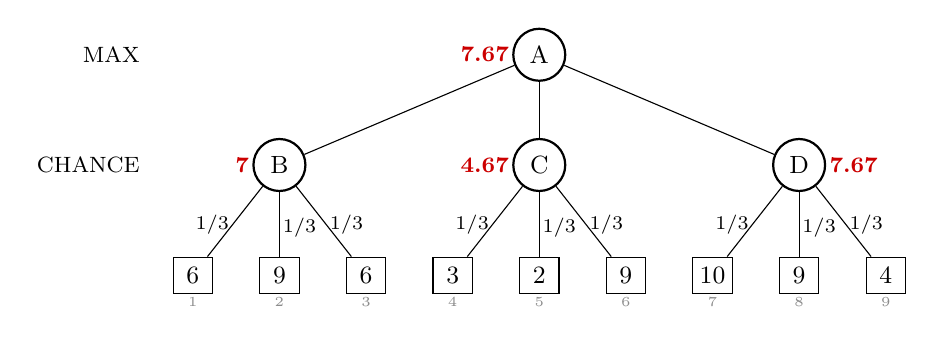
\begin{tikzpicture}[scale=1.0, every node/.style={transform shape}, gc/.style={draw, thick, circle, minimum size=6.6mm, inner sep=0pt, font=\small}, gl/.style={draw, rectangle, minimum width=5mm, minimum height=4.6mm, inner sep=1pt, font=\small}, gx/.style={draw=black!25, text=black!35}, val/.style={font=\footnotesize\bfseries, text=red!80!black, inner sep=1pt}]
\node[font=\footnotesize, anchor=east] at (-0.55,0.00) {MAX};
\node[font=\footnotesize, anchor=east] at (-0.55,-1.40) {CHANCE};
\node[gc, label={[val]left:7.67}] (n12) at (4.400,0.000) {A};
\node[gc, label={[val]left:7}] (n3) at (1.100,-1.400) {B};
\node[gl, label={[font=\tiny, text=black!45, inner sep=1pt]below:1}] (n0) at (0.000,-2.800) {6};
\node[gl, label={[font=\tiny, text=black!45, inner sep=1pt]below:2}] (n1) at (1.100,-2.800) {9};
\node[gl, label={[font=\tiny, text=black!45, inner sep=1pt]below:3}] (n2) at (2.200,-2.800) {6};
\node[gc, label={[val]left:4.67}] (n7) at (4.400,-1.400) {C};
\node[gl, label={[font=\tiny, text=black!45, inner sep=1pt]below:4}] (n4) at (3.300,-2.800) {3};
\node[gl, label={[font=\tiny, text=black!45, inner sep=1pt]below:5}] (n5) at (4.400,-2.800) {2};
\node[gl, label={[font=\tiny, text=black!45, inner sep=1pt]below:6}] (n6) at (5.500,-2.800) {9};
\node[gc, label={[val]right:7.67}] (n11) at (7.700,-1.400) {D};
\node[gl, label={[font=\tiny, text=black!45, inner sep=1pt]below:7}] (n8) at (6.600,-2.800) {10};
\node[gl, label={[font=\tiny, text=black!45, inner sep=1pt]below:8}] (n9) at (7.700,-2.800) {9};
\node[gl, label={[font=\tiny, text=black!45, inner sep=1pt]below:9}] (n10) at (8.800,-2.800) {4};
\draw (n12) -- (n3);
\draw (n12) -- (n7);
\draw (n12) -- (n11);
\draw (n3) -- (n0) node[pos=0.55, left, font=\scriptsize, inner sep=1pt]{$1/3$};
\draw (n3) -- (n1) node[pos=0.55, right, font=\scriptsize, inner sep=1pt]{$1/3$};
\draw (n3) -- (n2) node[pos=0.55, right, font=\scriptsize, inner sep=1pt]{$1/3$};
\draw (n7) -- (n4) node[pos=0.55, left, font=\scriptsize, inner sep=1pt]{$1/3$};
\draw (n7) -- (n5) node[pos=0.55, right, font=\scriptsize, inner sep=1pt]{$1/3$};
\draw (n7) -- (n6) node[pos=0.55, right, font=\scriptsize, inner sep=1pt]{$1/3$};
\draw (n11) -- (n8) node[pos=0.55, left, font=\scriptsize, inner sep=1pt]{$1/3$};
\draw (n11) -- (n9) node[pos=0.55, right, font=\scriptsize, inner sep=1pt]{$1/3$};
\draw (n11) -- (n10) node[pos=0.55, right, font=\scriptsize, inner sep=1pt]{$1/3$};
\end{tikzpicture}
\end{adjustbox}
\end{center}B $=7$, C $=14/3\approx4.67$, D $=23/3\approx7.67$; MAX chooses D.
\end{solbox}
\subq{(b)}Now assume every leaf value is at most 10 (and at least 0). Evaluating leaves left to right, identify the branches that can be pruned and explain each.
\begin{solbox}
After B, $\alpha=7$. At C, after leaves 3 and 2 the best possible value is $(3+2+10)/3=5\le7$ $\Rightarrow$ \textbf{prune leaf \#6}. At D, after 10 the bound is $10$, after 9 it is $9.67$, both $>7$, so leaf \#9 must be seen. Only leaf \#6 is pruned. Without an upper bound on the values no pruning is possible.
\end{solbox}
\question{7}Rollouts return 1 (win), 0.5 (draw) or 0 (loss) for the root player. Use $\mathrm{UCB1}=\bar V_i+C\sqrt{\ln N/n_i}$ (unvisited $=\infty$, ties to the left; a never-visited leaf is rolled out directly, otherwise all its children are added and the rollout starts at the first; $X_1\to X_3,X_4$ and $X_2\to X_5,X_6$ for $X\in\{A,B,C\}$). The current tree is:\begin{center}
\begin{adjustbox}{max width=\linewidth}
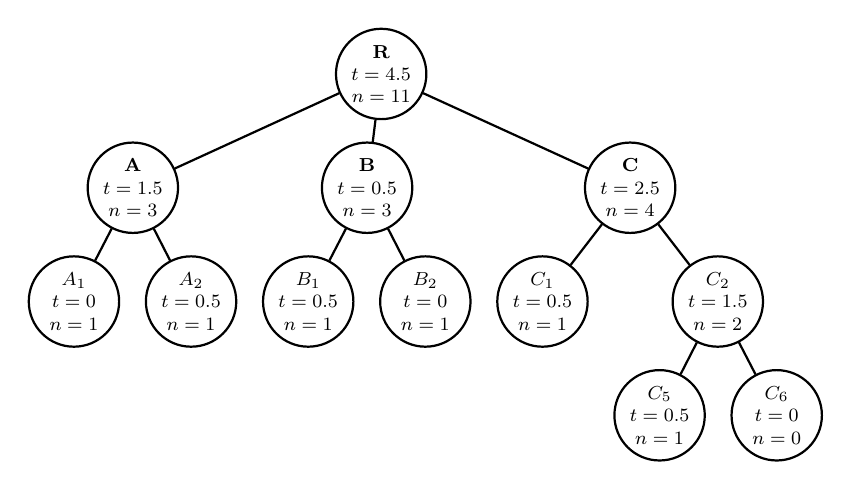
\begin{tikzpicture}[scale=0.85, every node/.style={transform shape}, mn/.style={draw, thick, circle, align=center, font=\footnotesize, inner sep=0.5pt, minimum size=13.5mm}]
\node[mn] (m1) at (4.59,0.00) {\textbf{R}\\ $t=4.5$\\ $n=11$};
\node[mn] (m2) at (0.88,-1.70) {\textbf{A}\\ $t=1.5$\\ $n=3$};
\node[mn] (m3) at (0.00,-3.40) {\textbf{$A_{1}$}\\ $t=0$\\ $n=1$};
\draw[thick] (m2) -- (m3);
\node[mn] (m4) at (1.75,-3.40) {\textbf{$A_{2}$}\\ $t=0.5$\\ $n=1$};
\draw[thick] (m2) -- (m4);
\draw[thick] (m1) -- (m2);
\node[mn] (m5) at (4.38,-1.70) {\textbf{B}\\ $t=0.5$\\ $n=3$};
\node[mn] (m6) at (3.50,-3.40) {\textbf{$B_{1}$}\\ $t=0.5$\\ $n=1$};
\draw[thick] (m5) -- (m6);
\node[mn] (m7) at (5.25,-3.40) {\textbf{$B_{2}$}\\ $t=0$\\ $n=1$};
\draw[thick] (m5) -- (m7);
\draw[thick] (m1) -- (m5);
\node[mn] (m8) at (8.31,-1.70) {\textbf{C}\\ $t=2.5$\\ $n=4$};
\node[mn] (m9) at (7.00,-3.40) {\textbf{$C_{1}$}\\ $t=0.5$\\ $n=1$};
\draw[thick] (m8) -- (m9);
\node[mn] (m10) at (9.62,-3.40) {\textbf{$C_{2}$}\\ $t=1.5$\\ $n=2$};
\node[mn] (m11) at (8.75,-5.10) {\textbf{$C_{5}$}\\ $t=0.5$\\ $n=1$};
\draw[thick] (m10) -- (m11);
\node[mn] (m12) at (10.50,-5.10) {\textbf{$C_{6}$}\\ $t=0$\\ $n=0$};
\draw[thick] (m10) -- (m12);
\draw[thick] (m8) -- (m10);
\draw[thick] (m1) -- (m8);
\end{tikzpicture}
\end{adjustbox}
\end{center}
\subq{(a)}With $C=\sqrt2$, calculate UCB1 of $A$, $B$, $C$. Which child is selected? For which values of $C$ would the root select $C$ instead of $A$?
\begin{solbox}
A: $\frac{1.5}{3} + \sqrt2\sqrt{\frac{\ln 11}{3}} = 1.764$; B: $\frac{0.5}{3} + \sqrt2\sqrt{\frac{\ln 11}{3}} = 1.431$; C: $\frac{2.5}{4} + \sqrt2\sqrt{\frac{\ln 11}{4}} = 1.720$ $\Rightarrow$ \textbf{A}. $C$ is preferred iff $0.625+c\sqrt{\ln 11/4}>0.5+c\sqrt{\ln 11/3}$, i.e.\ $c<\frac{0.625-0.5}{0.8940-0.7743}\approx\mathbf{1.04}$: a small constant favours exploitation (best average), a large one exploration of the less-visited $A$.
\end{solbox}
\subq{(b)}Perform three iterations whose rollouts return $0,\ 0.5,\ 0$ (in order); update the statistics and draw the final tree.
\begin{solbox}
\textbf{Iteration 1.}
\begin{itemize}[leftmargin=1.5em,itemsep=1pt]
\item \emph{Selection} at R ($N=11$): A: $\frac{1.5}{3} + \sqrt2\sqrt{\frac{\ln 11}{3}} = 1.764$; B: $\frac{0.5}{3} + \sqrt2\sqrt{\frac{\ln 11}{3}} = 1.431$; C: $\frac{2.5}{4} + \sqrt2\sqrt{\frac{\ln 11}{4}} = 1.720$ $\Rightarrow$ go to \textbf{A}.
\item \emph{Selection} at A ($N=3$): $A_{1}$: $\frac{0}{1} + \sqrt2\sqrt{\frac{\ln 3}{1}} = 1.482$; $A_{2}$: $\frac{0.5}{1} + \sqrt2\sqrt{\frac{\ln 3}{1}} = 1.982$ $\Rightarrow$ go to \textbf{$A_{2}$}.
\item \emph{Expansion}: $A_{2}$ was visited before ($n>0$) and has no children $\Rightarrow$ add $A_{5}$, $A_{6}$; roll out from the first one, \textbf{$A_{5}$}.
\item \emph{Simulation}: rollout from $A_{5}$ returns $0$.
\item \emph{Backpropagation}: add $0$ to $t$ and $1$ to $n$ for R $\to$ A $\to$ $A_{2}$ $\to$ $A_{5}$.
\end{itemize}
\textit{Statistics ($t/n$) after iteration 1:} R: 4.5/12, A: 1.5/4, $A_{1}$: 0/1, $A_{2}$: 0.5/2, $A_{5}$: 0/1, $A_{6}$: 0/0, B: 0.5/3, $B_{1}$: 0.5/1, $B_{2}$: 0/1, C: 2.5/4, $C_{1}$: 0.5/1, $C_{2}$: 1.5/2, $C_{5}$: 0.5/1, $C_{6}$: 0/0.

\smallskip
\textbf{Iteration 2.}
\begin{itemize}[leftmargin=1.5em,itemsep=1pt]
\item \emph{Selection} at R ($N=12$): A: $\frac{1.5}{4} + \sqrt2\sqrt{\frac{\ln 12}{4}} = 1.490$; B: $\frac{0.5}{3} + \sqrt2\sqrt{\frac{\ln 12}{3}} = 1.454$; C: $\frac{2.5}{4} + \sqrt2\sqrt{\frac{\ln 12}{4}} = 1.740$ $\Rightarrow$ go to \textbf{C}.
\item \emph{Selection} at C ($N=4$): $C_{1}$: $\frac{0.5}{1} + \sqrt2\sqrt{\frac{\ln 4}{1}} = 2.165$; $C_{2}$: $\frac{1.5}{2} + \sqrt2\sqrt{\frac{\ln 4}{2}} = 1.927$ $\Rightarrow$ go to \textbf{$C_{1}$}.
\item \emph{Expansion}: $C_{1}$ was visited before ($n>0$) and has no children $\Rightarrow$ add $C_{3}$, $C_{4}$; roll out from the first one, \textbf{$C_{3}$}.
\item \emph{Simulation}: rollout from $C_{3}$ returns $0.5$.
\item \emph{Backpropagation}: add $0.5$ to $t$ and $1$ to $n$ for R $\to$ C $\to$ $C_{1}$ $\to$ $C_{3}$.
\end{itemize}
\textit{Statistics ($t/n$) after iteration 2:} R: 5/13, A: 1.5/4, $A_{1}$: 0/1, $A_{2}$: 0.5/2, $A_{5}$: 0/1, $A_{6}$: 0/0, B: 0.5/3, $B_{1}$: 0.5/1, $B_{2}$: 0/1, C: 3/5, $C_{1}$: 1/2, $C_{3}$: 0.5/1, $C_{4}$: 0/0, $C_{2}$: 1.5/2, $C_{5}$: 0.5/1, $C_{6}$: 0/0.

\smallskip
\textbf{Iteration 3.}
\begin{itemize}[leftmargin=1.5em,itemsep=1pt]
\item \emph{Selection} at R ($N=13$): A: $\frac{1.5}{4} + \sqrt2\sqrt{\frac{\ln 13}{4}} = 1.507$; B: $\frac{0.5}{3} + \sqrt2\sqrt{\frac{\ln 13}{3}} = 1.474$; C: $\frac{3}{5} + \sqrt2\sqrt{\frac{\ln 13}{5}} = 1.613$ $\Rightarrow$ go to \textbf{C}.
\item \emph{Selection} at C ($N=5$): $C_{1}$: $\frac{1}{2} + \sqrt2\sqrt{\frac{\ln 5}{2}} = 1.769$; $C_{2}$: $\frac{1.5}{2} + \sqrt2\sqrt{\frac{\ln 5}{2}} = 2.019$ $\Rightarrow$ go to \textbf{$C_{2}$}.
\item \emph{Selection} at $C_{2}$ ($N=2$): $C_{5}$: $\frac{0.5}{1} + \sqrt2\sqrt{\frac{\ln 2}{1}} = 1.677$; $C_{6}$: $\infty$ (unvisited) $\Rightarrow$ go to \textbf{$C_{6}$}.
\item \emph{Expansion}: none --- \textbf{$C_{6}$} has $n=0$, so we roll out directly from it.
\item \emph{Simulation}: rollout from $C_{6}$ returns $0$.
\item \emph{Backpropagation}: add $0$ to $t$ and $1$ to $n$ for R $\to$ C $\to$ $C_{2}$ $\to$ $C_{6}$.
\end{itemize}
\textit{Statistics ($t/n$) after iteration 3:} R: 5/14, A: 1.5/4, $A_{1}$: 0/1, $A_{2}$: 0.5/2, $A_{5}$: 0/1, $A_{6}$: 0/0, B: 0.5/3, $B_{1}$: 0.5/1, $B_{2}$: 0/1, C: 3/6, $C_{1}$: 1/2, $C_{3}$: 0.5/1, $C_{4}$: 0/0, $C_{2}$: 1.5/3, $C_{5}$: 0.5/1, $C_{6}$: 0/1.\par Final tree:\begin{center}
\begin{adjustbox}{max width=\linewidth}
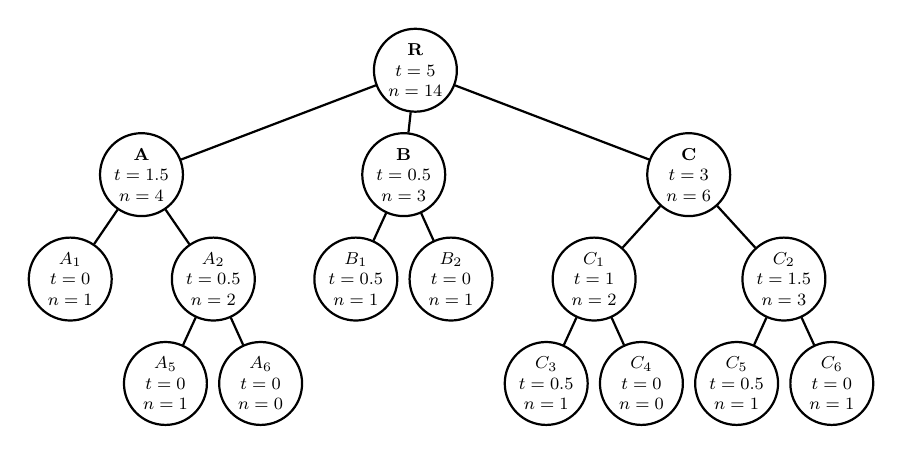
\begin{tikzpicture}[scale=0.78, every node/.style={transform shape}, mn/.style={draw, thick, circle, align=center, font=\footnotesize, inner sep=0.5pt, minimum size=13.5mm}]
\node[mn] (m1) at (5.62,0.00) {\textbf{R}\\ $t=5$\\ $n=14$};
\node[mn] (m2) at (1.16,-1.70) {\textbf{A}\\ $t=1.5$\\ $n=4$};
\node[mn] (m3) at (0.00,-3.40) {\textbf{$A_{1}$}\\ $t=0$\\ $n=1$};
\draw[thick] (m2) -- (m3);
\node[mn] (m4) at (2.33,-3.40) {\textbf{$A_{2}$}\\ $t=0.5$\\ $n=2$};
\node[mn] (m5) at (1.55,-5.10) {\textbf{$A_{5}$}\\ $t=0$\\ $n=1$};
\draw[thick] (m4) -- (m5);
\node[mn] (m6) at (3.10,-5.10) {\textbf{$A_{6}$}\\ $t=0$\\ $n=0$};
\draw[thick] (m4) -- (m6);
\draw[thick] (m2) -- (m4);
\draw[thick] (m1) -- (m2);
\node[mn] (m7) at (5.43,-1.70) {\textbf{B}\\ $t=0.5$\\ $n=3$};
\node[mn] (m8) at (4.65,-3.40) {\textbf{$B_{1}$}\\ $t=0.5$\\ $n=1$};
\draw[thick] (m7) -- (m8);
\node[mn] (m9) at (6.20,-3.40) {\textbf{$B_{2}$}\\ $t=0$\\ $n=1$};
\draw[thick] (m7) -- (m9);
\draw[thick] (m1) -- (m7);
\node[mn] (m10) at (10.07,-1.70) {\textbf{C}\\ $t=3$\\ $n=6$};
\node[mn] (m11) at (8.53,-3.40) {\textbf{$C_{1}$}\\ $t=1$\\ $n=2$};
\node[mn] (m12) at (7.75,-5.10) {\textbf{$C_{3}$}\\ $t=0.5$\\ $n=1$};
\draw[thick] (m11) -- (m12);
\node[mn] (m13) at (9.30,-5.10) {\textbf{$C_{4}$}\\ $t=0$\\ $n=0$};
\draw[thick] (m11) -- (m13);
\draw[thick] (m10) -- (m11);
\node[mn] (m14) at (11.62,-3.40) {\textbf{$C_{2}$}\\ $t=1.5$\\ $n=3$};
\node[mn] (m15) at (10.85,-5.10) {\textbf{$C_{5}$}\\ $t=0.5$\\ $n=1$};
\draw[thick] (m14) -- (m15);
\node[mn] (m16) at (12.40,-5.10) {\textbf{$C_{6}$}\\ $t=0$\\ $n=1$};
\draw[thick] (m14) -- (m16);
\draw[thick] (m10) -- (m14);
\draw[thick] (m1) -- (m10);
\end{tikzpicture}
\end{adjustbox}
\end{center}
\end{solbox}
\question{8}This problem is about map colouring. Each region must be coloured Red (R), Green (G) or Blue (B), and neighbouring regions must have different colours. The constraint graph is shown below. The following questions are mutually independent.\begin{center}
\begin{adjustbox}{max width=\linewidth}
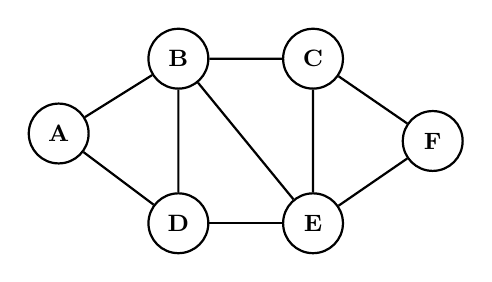
\begin{tikzpicture}[scale=0.95, every node/.style={transform shape}, cv/.style={draw, thick, circle, minimum size=8mm, inner sep=0pt, font=\small\bfseries}]
\node[cv] (A) at (0.00,1.20) {A};
\node[cv] (B) at (1.60,2.20) {B};
\node[cv] (C) at (3.40,2.20) {C};
\node[cv] (D) at (1.60,0.00) {D};
\node[cv] (E) at (3.40,0.00) {E};
\node[cv] (F) at (5.00,1.10) {F};
\draw[thick] (A) to[] (B);
\draw[thick] (A) to[] (D);
\draw[thick] (B) to[] (C);
\draw[thick] (B) to[] (D);
\draw[thick] (B) to[] (E);
\draw[thick] (C) to[] (E);
\draw[thick] (C) to[] (F);
\draw[thick] (D) to[] (E);
\draw[thick] (E) to[] (F);
\end{tikzpicture}
\end{adjustbox}
\end{center}
\subq{(a)}\textbf{Cross out} all values that would be eliminated by \emph{forward checking} after variable B has been assigned as shown.\begin{center}\small\begin{tabular}{|l|c|c|c|c|c|c|}\hline Variables & \textbf{A} & \textbf{B} & \textbf{C} & \textbf{D} & \textbf{E} & \textbf{F}\\ \hline Domains & R\ G\ B & \textbf{R} & R\ G\ B & R\ G\ B & R\ G\ B & R\ G\ B\\ \hline\end{tabular}\end{center}
\begin{solbox}
\begin{center}\small\begin{tabular}{|l|c|c|c|c|c|c|}\hline Variables & \textbf{A} & \textbf{B} & \textbf{C} & \textbf{D} & \textbf{E} & \textbf{F}\\ \hline Domains & \textcolor{red!70!black}{\sout{R}}\ G\ B & \textbf{R}\ \textcolor{red!70!black}{\sout{G}}\ \textcolor{red!70!black}{\sout{B}} & \textcolor{red!70!black}{\sout{R}}\ G\ B & \textcolor{red!70!black}{\sout{R}}\ G\ B & \textcolor{red!70!black}{\sout{R}}\ G\ B & R\ G\ B\\ \hline\end{tabular}\end{center}Only the neighbours of B (A, C, D, E) lose R.
\end{solbox}
\subq{(b)}A and B have been assigned as shown, but no constraint propagation has been done yet. \textbf{Cross out} all values that would be eliminated by \emph{arc consistency} (AC-3).\begin{center}\small\begin{tabular}{|l|c|c|c|c|c|c|}\hline Variables & \textbf{A} & \textbf{B} & \textbf{C} & \textbf{D} & \textbf{E} & \textbf{F}\\ \hline Domains & \textbf{R} & \textbf{G} & R\ G\ B & R\ G\ B & R\ G\ B & R\ G\ B\\ \hline\end{tabular}\end{center}
\begin{solbox}
\begin{center}\small\begin{tabular}{|l|c|c|c|c|c|c|}\hline Variables & \textbf{A} & \textbf{B} & \textbf{C} & \textbf{D} & \textbf{E} & \textbf{F}\\ \hline Domains & \textbf{R}\ \textcolor{red!70!black}{\sout{G}}\ \textcolor{red!70!black}{\sout{B}} & \textcolor{red!70!black}{\sout{R}}\ \textbf{G}\ \textcolor{red!70!black}{\sout{B}} & \textcolor{red!70!black}{\sout{R}}\ \textcolor{red!70!black}{\sout{G}}\ B & \textcolor{red!70!black}{\sout{R}}\ \textcolor{red!70!black}{\sout{G}}\ B & R\ \textcolor{red!70!black}{\sout{G}}\ \textcolor{red!70!black}{\sout{B}} & \textcolor{red!70!black}{\sout{R}}\ G\ \textcolor{red!70!black}{\sout{B}}\\ \hline\end{tabular}\end{center}Propagation continues through the graph (unlike forward checking): every arc $X_i\to X_j$ is revised until no domain changes. Here arc consistency even leaves a single value for every variable.
\end{solbox}
\subq{(c)}Variable A is already assigned and constraint propagation has been done. \textbf{Circle} all unassigned variables that might be selected by the \emph{Minimum-Remaining-Values} (MRV) heuristic.\begin{center}\small\begin{tabular}{|l|c|c|c|c|c|c|}\hline Variables & \textbf{A} & \textbf{B} & \textbf{C} & \textbf{D} & \textbf{E} & \textbf{F}\\ \hline Domains & \textbf{R} & G\ B & R\ G\ B & G\ B & R\ G\ B & R\ G\ B\\ \hline\end{tabular}\end{center}
\begin{solbox}
Remaining values: B: 2, C: 3, D: 2, E: 3, F: 3 $\Rightarrow$ MRV may select \textbf{B, D}.
\end{solbox}
\subq{(d)}Same situation. \textbf{Circle} all unassigned variables that might be selected by the \emph{Degree Heuristic}.\begin{center}\small\begin{tabular}{|l|c|c|c|c|c|c|}\hline Variables & \textbf{A} & \textbf{B} & \textbf{C} & \textbf{D} & \textbf{E} & \textbf{F}\\ \hline Domains & \textbf{R} & G\ B & R\ G\ B & G\ B & R\ G\ B & R\ G\ B\\ \hline\end{tabular}\end{center}
\begin{solbox}
Degree = number of constraints with other \emph{unassigned} variables: B: 3, C: 3, D: 2, E: 4, F: 2 $\Rightarrow$ the degree heuristic may select \textbf{E}.
\end{solbox}
\subq{(e)}Assume no variable has been assigned yet. Solve the CSP using backtracking with \emph{forward checking}, choosing variables with MRV, then the degree heuristic (DH), and finally alphabetical order; try values in the order R, G, B. For every step give the MRV value of every region not yet coloured, and the DH values of the regions tied on the minimum MRV.
\begin{solbox}
\par \underline{Step 1}\par\begin{center}\small \begin{tabular}{|l|c|c|c|c|c|c|}\hline Variables & \textbf{A} & \textbf{B} & \textbf{C} & \textbf{D} & \textbf{E} & \textbf{F}\\ \hline MRV & \textcolor{blue!60!black}{3} & \textcolor{blue!60!black}{3} & \textcolor{blue!60!black}{3} & \textcolor{blue!60!black}{3} & \textcolor{blue!60!black}{3} & \textcolor{blue!60!black}{3}\\ \hline DH & \textcolor{blue!60!black}{2} & \textcolor{blue!60!black}{4} & \textcolor{blue!60!black}{3} & \textcolor{blue!60!black}{3} & \textcolor{blue!60!black}{4} & \textcolor{blue!60!black}{2}\\ \hline\end{tabular}\end{center}Assign to the variable \textbf{B} with the value \textbf{R} (tie on MRV and DH, broken alphabetically). Domains before this step: A=RGB, B=RGB, C=RGB, D=RGB, E=RGB, F=RGB.\par
\underline{Step 2}\par\begin{center}\small \begin{tabular}{|l|c|c|c|c|c|c|}\hline Variables & \textbf{A} & \textbf{B} & \textbf{C} & \textbf{D} & \textbf{E} & \textbf{F}\\ \hline MRV & \textcolor{blue!60!black}{2} & -- & \textcolor{blue!60!black}{2} & \textcolor{blue!60!black}{2} & \textcolor{blue!60!black}{2} & \textcolor{blue!60!black}{3}\\ \hline DH & \textcolor{blue!60!black}{1} &  & \textcolor{blue!60!black}{2} & \textcolor{blue!60!black}{2} & \textcolor{blue!60!black}{3} & \\ \hline\end{tabular}\end{center}Assign to the variable \textbf{E} with the value \textbf{G} (tie on MRV broken by DH). Domains before this step: A=GB, B=R, C=GB, D=GB, E=GB, F=RGB.\par
\underline{Step 3}\par\begin{center}\small \begin{tabular}{|l|c|c|c|c|c|c|}\hline Variables & \textbf{A} & \textbf{B} & \textbf{C} & \textbf{D} & \textbf{E} & \textbf{F}\\ \hline MRV & \textcolor{blue!60!black}{2} & -- & \textcolor{blue!60!black}{1} & \textcolor{blue!60!black}{1} & -- & \textcolor{blue!60!black}{2}\\ \hline DH &  &  & \textcolor{blue!60!black}{1} & \textcolor{blue!60!black}{1} &  & \\ \hline\end{tabular}\end{center}Assign to the variable \textbf{C} with the value \textbf{B} (tie on MRV and DH, broken alphabetically). Domains before this step: A=GB, B=R, C=B, D=B, E=G, F=RB.\par
\underline{Step 4}\par\begin{center}\small \begin{tabular}{|l|c|c|c|c|c|c|}\hline Variables & \textbf{A} & \textbf{B} & \textbf{C} & \textbf{D} & \textbf{E} & \textbf{F}\\ \hline MRV & \textcolor{blue!60!black}{2} & -- & -- & \textcolor{blue!60!black}{1} & -- & \textcolor{blue!60!black}{1}\\ \hline DH &  &  &  & \textcolor{blue!60!black}{1} &  & \textcolor{blue!60!black}{0}\\ \hline\end{tabular}\end{center}Assign to the variable \textbf{D} with the value \textbf{B} (tie on MRV broken by DH). Domains before this step: A=GB, B=R, C=B, D=B, E=G, F=R.\par
\underline{Step 5}\par\begin{center}\small \begin{tabular}{|l|c|c|c|c|c|c|}\hline Variables & \textbf{A} & \textbf{B} & \textbf{C} & \textbf{D} & \textbf{E} & \textbf{F}\\ \hline MRV & \textcolor{blue!60!black}{1} & -- & -- & -- & -- & \textcolor{blue!60!black}{1}\\ \hline DH & \textcolor{blue!60!black}{0} &  &  &  &  & \textcolor{blue!60!black}{0}\\ \hline\end{tabular}\end{center}Assign to the variable \textbf{A} with the value \textbf{G} (tie on MRV and DH, broken alphabetically). Domains before this step: A=G, B=R, C=B, D=B, E=G, F=R.\par
\underline{Step 6}\par\begin{center}\small \begin{tabular}{|l|c|c|c|c|c|c|}\hline Variables & \textbf{A} & \textbf{B} & \textbf{C} & \textbf{D} & \textbf{E} & \textbf{F}\\ \hline MRV & -- & -- & -- & -- & -- & \textcolor{blue!60!black}{1}\\ \hline DH &  &  &  &  &  & \\ \hline\end{tabular}\end{center}Assign to the variable \textbf{F} with the value \textbf{R} (unique minimum MRV). Domains before this step: A=G, B=R, C=B, D=B, E=G, F=R.\par Solution: A=G, B=R, C=B, D=B, E=G, F=R. No backtracking is needed.
\end{solbox}
\question{9}Cryptarithmetic: $\;\begin{array}{r} T\,O\\ +\;G\,O\\ \hline O\,U\,T\end{array}\;$ --- distinct letters are distinct digits and leading digits are non-zero.
\subq{(a)}Formulate the CSP: variables (including carries), domains and constraints.
\begin{solbox}
Variables $T,O,G,U$, carries $C_1,C_2$; domains $\{0..9\}$, carries $\{0,1\}$. Constraints: Alldiff$(T,O,G,U)$; $O+O=T+10C_1$; $C_1+T+G=U+10C_2$; $C_2=O$; $T,G,O\neq0$.
\end{solbox}
\subq{(b)}Solve it by constraint propagation, explaining each deduction.
\begin{solbox}
$O=C_2\in\{0,1\}$, $O\ne0$ $\Rightarrow O=1$. $2=T+10C_1\Rightarrow T=2, C_1=0$. $2+G=U+10\Rightarrow G=U+8$, so $(G,U)\in\{(8,0),(9,1)\}$; $U=1$ clashes with $O$ $\Rightarrow G=8,U=0$: \textbf{21 + 81 = 102}.
\end{solbox}
\question{10}\textit{Lab scheduling.} Five lab sessions must each be run by one TA, and a TA cannot run two overlapping sessions: P1 8:00--9:30, P2 9:00--10:30, P3 9:30--11:00, P4 10:30--12:00, P5 11:30--13:00 (sessions that only touch do not overlap). TA \textbf{H} can run P1, P2, P4, P5; \textbf{L} can run P2, P3; \textbf{M} can run P1, P3, P4.
\subq{(a)}Formulate the CSP (one variable per session; apply the availability constraints to the domains) and draw the constraint graph.
\begin{solbox}
\begin{center}\small\begin{tabular}{|l|c|c|c|c|c|}\hline Variables & \textbf{P1} & \textbf{P2} & \textbf{P3} & \textbf{P4} & \textbf{P5}\\ \hline Domains & H, M & H, L & L, M & H, M & H\\ \hline\end{tabular}\end{center}Binary constraints: $P1\ne P2$, $P2\ne P3$, $P3\ne P4$, $P4\ne P5$\begin{center}
\begin{adjustbox}{max width=\linewidth}
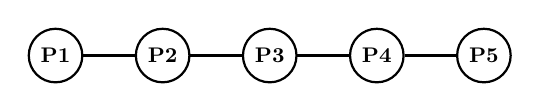
\begin{tikzpicture}[scale=0.85, every node/.style={transform shape}, cv/.style={draw, thick, circle, minimum size=8mm, inner sep=0pt, font=\small\bfseries}]
\node[cv] (P1) at (0.00,0.00) {P1};
\node[cv] (P2) at (1.60,0.00) {P2};
\node[cv] (P3) at (3.20,0.00) {P3};
\node[cv] (P4) at (4.80,0.00) {P4};
\node[cv] (P5) at (6.40,0.00) {P5};
\draw[thick] (P1) to[] (P2);
\draw[thick] (P2) to[] (P3);
\draw[thick] (P3) to[] (P4);
\draw[thick] (P4) to[] (P5);
\end{tikzpicture}
\end{adjustbox}
\end{center}
\end{solbox}
\subq{(b)}Run AC-3 with the initial queue $P1\to P2$, $P2\to P1$, $P2\to P3$, $P3\to P2$, $P3\to P4$, $P4\to P3$, $P4\to P5$, $P5\to P4$. Cross out the values it eliminates from your domains in (a), and give the solution.
\begin{solbox}
\begin{center}\small\begin{tabular}{c c c l p{5cm}}\toprule
\# & Arc popped & Removed from tail & New domain & Arcs appended to queue \\ \midrule
1 & $P1 \to P2$ & -- &  & -- \\
2 & $P2 \to P1$ & -- &  & -- \\
3 & $P2 \to P3$ & -- &  & -- \\
4 & $P3 \to P2$ & -- &  & -- \\
5 & $P3 \to P4$ & -- &  & -- \\
6 & $P4 \to P3$ & -- &  & -- \\
7 & $P4 \to P5$ & H & $D_{P4}=\{M\}$ & $P3\to P4$ \\
8 & $P5 \to P4$ & -- &  & -- \\
9 & $P3 \to P4$ & M & $D_{P3}=\{L\}$ & $P2\to P3$ \\
10 & $P2 \to P3$ & L & $D_{P2}=\{H\}$ & $P1\to P2$ \\
11 & $P1 \to P2$ & H & $D_{P1}=\{M\}$ & -- \\
\bottomrule\end{tabular}\end{center}\begin{center}\small\begin{tabular}{|l|c|c|c|c|c|}\hline Variables & \textbf{P1} & \textbf{P2} & \textbf{P3} & \textbf{P4} & \textbf{P5}\\ \hline Domains & \textcolor{red!70!black}{\sout{H}}\ M & H\ \textcolor{red!70!black}{\sout{L}} & L\ \textcolor{red!70!black}{\sout{M}} & \textcolor{red!70!black}{\sout{H}}\ M & H\\ \hline\end{tabular}\end{center}Every domain becomes a singleton: P1=M, P2=H, P3=L, P4=M, P5=H.
\end{solbox}
\question{11}Answer the following questions briefly.
\subq{(a)}Match each field with its contribution to AI: (1) Philosophy, (2) Mathematics, (3) Economics, (4) Neuroscience, (5) Psychology, (6) Control theory. (a) neurons as information-processing units; (b) utility and decision theory; (c) logic, reasoning, mind as a physical system; (d) maximising an objective function over time; (e) formal proof, algorithms, (in)tractability, probability; (f) how people perceive, process information and represent knowledge.
\begin{solbox}
(1)c, (2)e, (3)b, (4)a, (5)f, (6)d.
\end{solbox}
\subq{(b)}Order chronologically and explain the AI winter: Deep Blue beats Kasparov; Dartmouth meeting; McCulloch \& Pitts; AlphaGo beats Lee Sedol; Turing's ``Computing Machinery and Intelligence''; the expert-systems boom.
\begin{solbox}
1943 McCulloch \& Pitts, 1950 Turing, 1956 Dartmouth, 1980--88 expert-systems boom, 1997 Deep Blue, 2016 AlphaGo. The AI winter (1988--93) was the bust after the expert-systems boom, when expectations were not met and funding collapsed.
\end{solbox}
\subq{(c)}For the 8-puzzle below compute $h_1$ (misplaced tiles) and $h_2$ (total Manhattan distance). Which heuristic dominates the other, and what does dominance imply for A*?\par\begin{center}Start: {\renewcommand{\arraystretch}{1.3}\begin{tabular}{|c|c|c|}\hline 4 & 1 & 2 \\ \hline
 & 8 & 7 \\ \hline
6 & 3 & 5 \\ \hline\end{tabular}}\qquad Goal: {\renewcommand{\arraystretch}{1.3}\begin{tabular}{|c|c|c|}\hline  & 1 & 2 \\ \hline
3 & 4 & 5 \\ \hline
6 & 7 & 8 \\ \hline\end{tabular}}\end{center}
\begin{solbox}
$h_1=\mathbf{5}$ (tiles 3, 4, 5, 7, 8); $h_2=\mathbf{9}$ (1:0, 2:0, 3:2, 4:2, 5:1, 6:0, 7:2, 8:2). $h_2$ dominates $h_1$: every misplaced tile is at Manhattan distance $\ge1$, so $h_2(n)\ge h_1(n)$ for all $n$. With both consistent, A* using $h_2$ never expands more nodes than A* using $h_1$, since every node surely expanded with $h_2$ ($f<C^*$) is also surely expanded with $h_1$.
\end{solbox}
\subq{(d)}A CSP has $n=5$ variables with domain size $d=3$. How many leaves does a naive search tree (any unassigned variable at each level) have, and how many with backtracking? Which property justifies the difference?
\begin{solbox}
Naive: $n!\,d^n=120\cdot243=\mathbf{29{,}160}$ leaves for only $d^n=243$ complete assignments. Assignments are \textbf{commutative}, so backtracking fixes one variable per level: $d^n=\mathbf{243}$ leaves.
\end{solbox}
\question{12}True or false?
For each statement, circle \textbf{T} or \textbf{F} and justify your answer in one or two sentences (an answer without a correct justification earns no credit).
\subq{1.}Uniform-cost search expands nodes in order of their optimal path cost. \hfill \textbf{T \quad F}
\begin{solbox}
\T. By the separation property, the first time a state is expanded its $g$ is optimal (positive costs).
\end{solbox}
\subq{2.}A* is optimally efficient among optimal algorithms using the same heuristic. \hfill \textbf{T \quad F}
\begin{solbox}
\T. Any such algorithm must expand all nodes with $f<C^*$, otherwise it could miss the optimum.
\end{solbox}
\subq{3.}If $h(n)=0$ for every node, A* behaves exactly like UCS. \hfill \textbf{T \quad F}
\begin{solbox}
\T. $f=g+0=g$.
\end{solbox}
\subq{4.}If $h_2$ dominates $h_1$ and both are consistent, A* with $h_2$ never expands more nodes than A* with $h_1$ (ignoring ties). \hfill \textbf{T \quad F}
\begin{solbox}
\T. $h_1\le h_2<C^*-g$ for every node surely expanded with $h_2$.
\end{solbox}
\subq{5.}Local beam search with $k$ states is the same as $k$ independent random-restart hill climbs run in parallel. \hfill \textbf{T \quad F}
\begin{solbox}
\F. The $k$ best successors are chosen from the pooled list, so information passes between the threads.
\end{solbox}
\subq{6.}The amount of alpha-beta pruning does not depend on the move ordering. \hfill \textbf{T \quad F}
\begin{solbox}
\F. Perfect ordering gives $O(b^{m/2})$, random about $O(b^{3m/4})$, the worst ordering no pruning at all.
\end{solbox}
\subq{7.}Against a sub-optimal MIN player, the minimax move always gives MAX the best possible outcome. \hfill \textbf{T \quad F}
\begin{solbox}
\F. MAX does at least as well as against an optimal MIN, but a riskier move may do better.
\end{solbox}
\subq{8.}MCTS grows its tree symmetrically, level by level. \hfill \textbf{T \quad F}
\begin{solbox}
\F. It grows asymmetrically towards the more promising moves.
\end{solbox}
\subq{9.}Node consistency concerns binary constraints. \hfill \textbf{T \quad F}
\begin{solbox}
\F. It concerns unary constraints; arc consistency handles binary ones.
\end{solbox}
\subq{10.}The degree heuristic is mainly used as a tie-breaker for MRV. \hfill \textbf{T \quad F}
\begin{solbox}
\T. At the start all domains are full, so MRV ties and degree decides.
\end{solbox}
\end{document}